\documentclass[11pt]{article}

\bibliographystyle{elsarticle-num}

\usepackage{amsmath,amsfonts,graphicx,microtype}
\usepackage[margin=1in]{geometry}

\newcommand{\p}{\partial}
\newcommand{\bxi}{\boldsymbol\xi}
\newcommand{\bsig}{\boldsymbol\sigma}
\newcommand{\bOmega}{\boldsymbol\Omega}
\newcommand{\mcD}{\mathcal{D}}
\newcommand{\bC}{\mathbf{C}}
\newcommand{\bD}{\mathbf{D}}
\newcommand{\bL}{\mathbf{L}}
\newcommand{\bT}{\mathbf{T}}
\newcommand{\bU}{\mathbf{U}}
\newcommand{\bX}{\mathbf{X}}
\newcommand{\bx}{\mathbf{x}}
\newcommand{\bu}{\mathbf{u}}
\newcommand{\Trans}{\mathsf{T}}
\newcommand{\Dpl}{D^\text{pl}}
\newcommand{\bDel}{\bD^\text{el}}
\newcommand{\bDpl}{\bD^\text{pl}}
\newcommand{\bgrad}{\boldsymbol{\nabla}}
\newcommand{\adv}{\left(\bU\cdot\bgrad\right)}
\newcommand{\advn}{\left(\bU_n\cdot\bgrad\right)}
\newcommand{\bA}{\mathbf{A}}
\newcommand{\bB}{\mathbf{B}}
\newcommand{\dVdX}{\frac{\p V}{\p X}}
\newcommand{\dVdY}{\frac{\p V}{\p Y}}
\newcommand{\dUdX}{\frac{\p U}{\p X}}
\newcommand{\dUdY}{\frac{\p U}{\p Y}}
\newcommand{\dVndX}{\frac{\p V_n}{\p X}}
\newcommand{\dVndY}{\frac{\p V_n}{\p Y}}
\newcommand{\dUndX}{\frac{\p U_n}{\p X}}
\newcommand{\dUndY}{\frac{\p U_n}{\p Y}}
\newcommand{\dvdx}{\frac{\p v}{\p x}}
\newcommand{\dvdy}{\frac{\p v}{\p y}}
\newcommand{\dudx}{\frac{\p u}{\p x}}
\newcommand{\dudy}{\frac{\p u}{\p y}}
\newcommand{\dUdt}{\frac{\p U}{\p t}}
\newcommand{\dpdX}{\frac{\p p}{\p X}}
\newcommand{\dpdY}{\frac{\p p}{\p Y}}
\newcommand{\dqdX}{\frac{\p q}{\p X}}
\newcommand{\dqdY}{\frac{\p q}{\p Y}}
\newcommand{\dsdX}{\frac{\p s}{\p X}}
\newcommand{\dsdY}{\frac{\p s}{\p Y}}
\newcommand{\dtaudX}{\frac{\p \tau}{\p X}}
\newcommand{\dtaudY}{\frac{\p \tau}{\p Y}}
\newcommand{\sbar}{\bar{s}}


\renewcommand{\arraystretch}{1.1}

% Set-up for hypertext references
\usepackage{hyperref,color}
\definecolor{webgreen}{rgb}{0,.35,0}
\definecolor{webbrown}{rgb}{.6,0,0}
\definecolor{RoyalBlue}{rgb}{0,0,0.9}
\hypersetup{
   colorlinks=true, linktocpage=true, pdfstartpage=3, pdfstartview=FitV,
   breaklinks=true, pdfpagemode=UseNone, pageanchor=true, pdfpagemode=UseOutlines,
   plainpages=false, bookmarksnumbered, bookmarksopen=true, bookmarksopenlevel=1,
   hypertexnames=true, pdfhighlight=/O,
   urlcolor=webbrown, linkcolor=RoyalBlue, citecolor=webgreen,
   pdfauthor={Nicholas Boffi},
   pdftitle={Bar Coordinate Transformations},
   pdfsubject={},
   pdfkeywords={},
   pdfcreator={pdfLaTeX},
   pdfproducer={LaTeX with hyperref}
}

\begin{document}

\title{Bar Coordinate Transformations}
\author{Nicholas Boffi}
\maketitle

\section*{Problem 1}
Assume that we have some biaxial deformation of a reference configuration such that we can write down the spatial coordinates at any given time as
\begin{align}
    x(t) &= A(t)X,\\
    y(t) &= B(t)Y.
    \label{eqn:coords}
\end{align}
Here, $X$ and $Y$ are the coordinates in the reference configuration and $A(t)$ and $B(t)$ describe the biaxial stretching. This is depicted in the accompanying figure, Fig.~\ref{fig:prob1}.
\begin{figure}
    \centering
    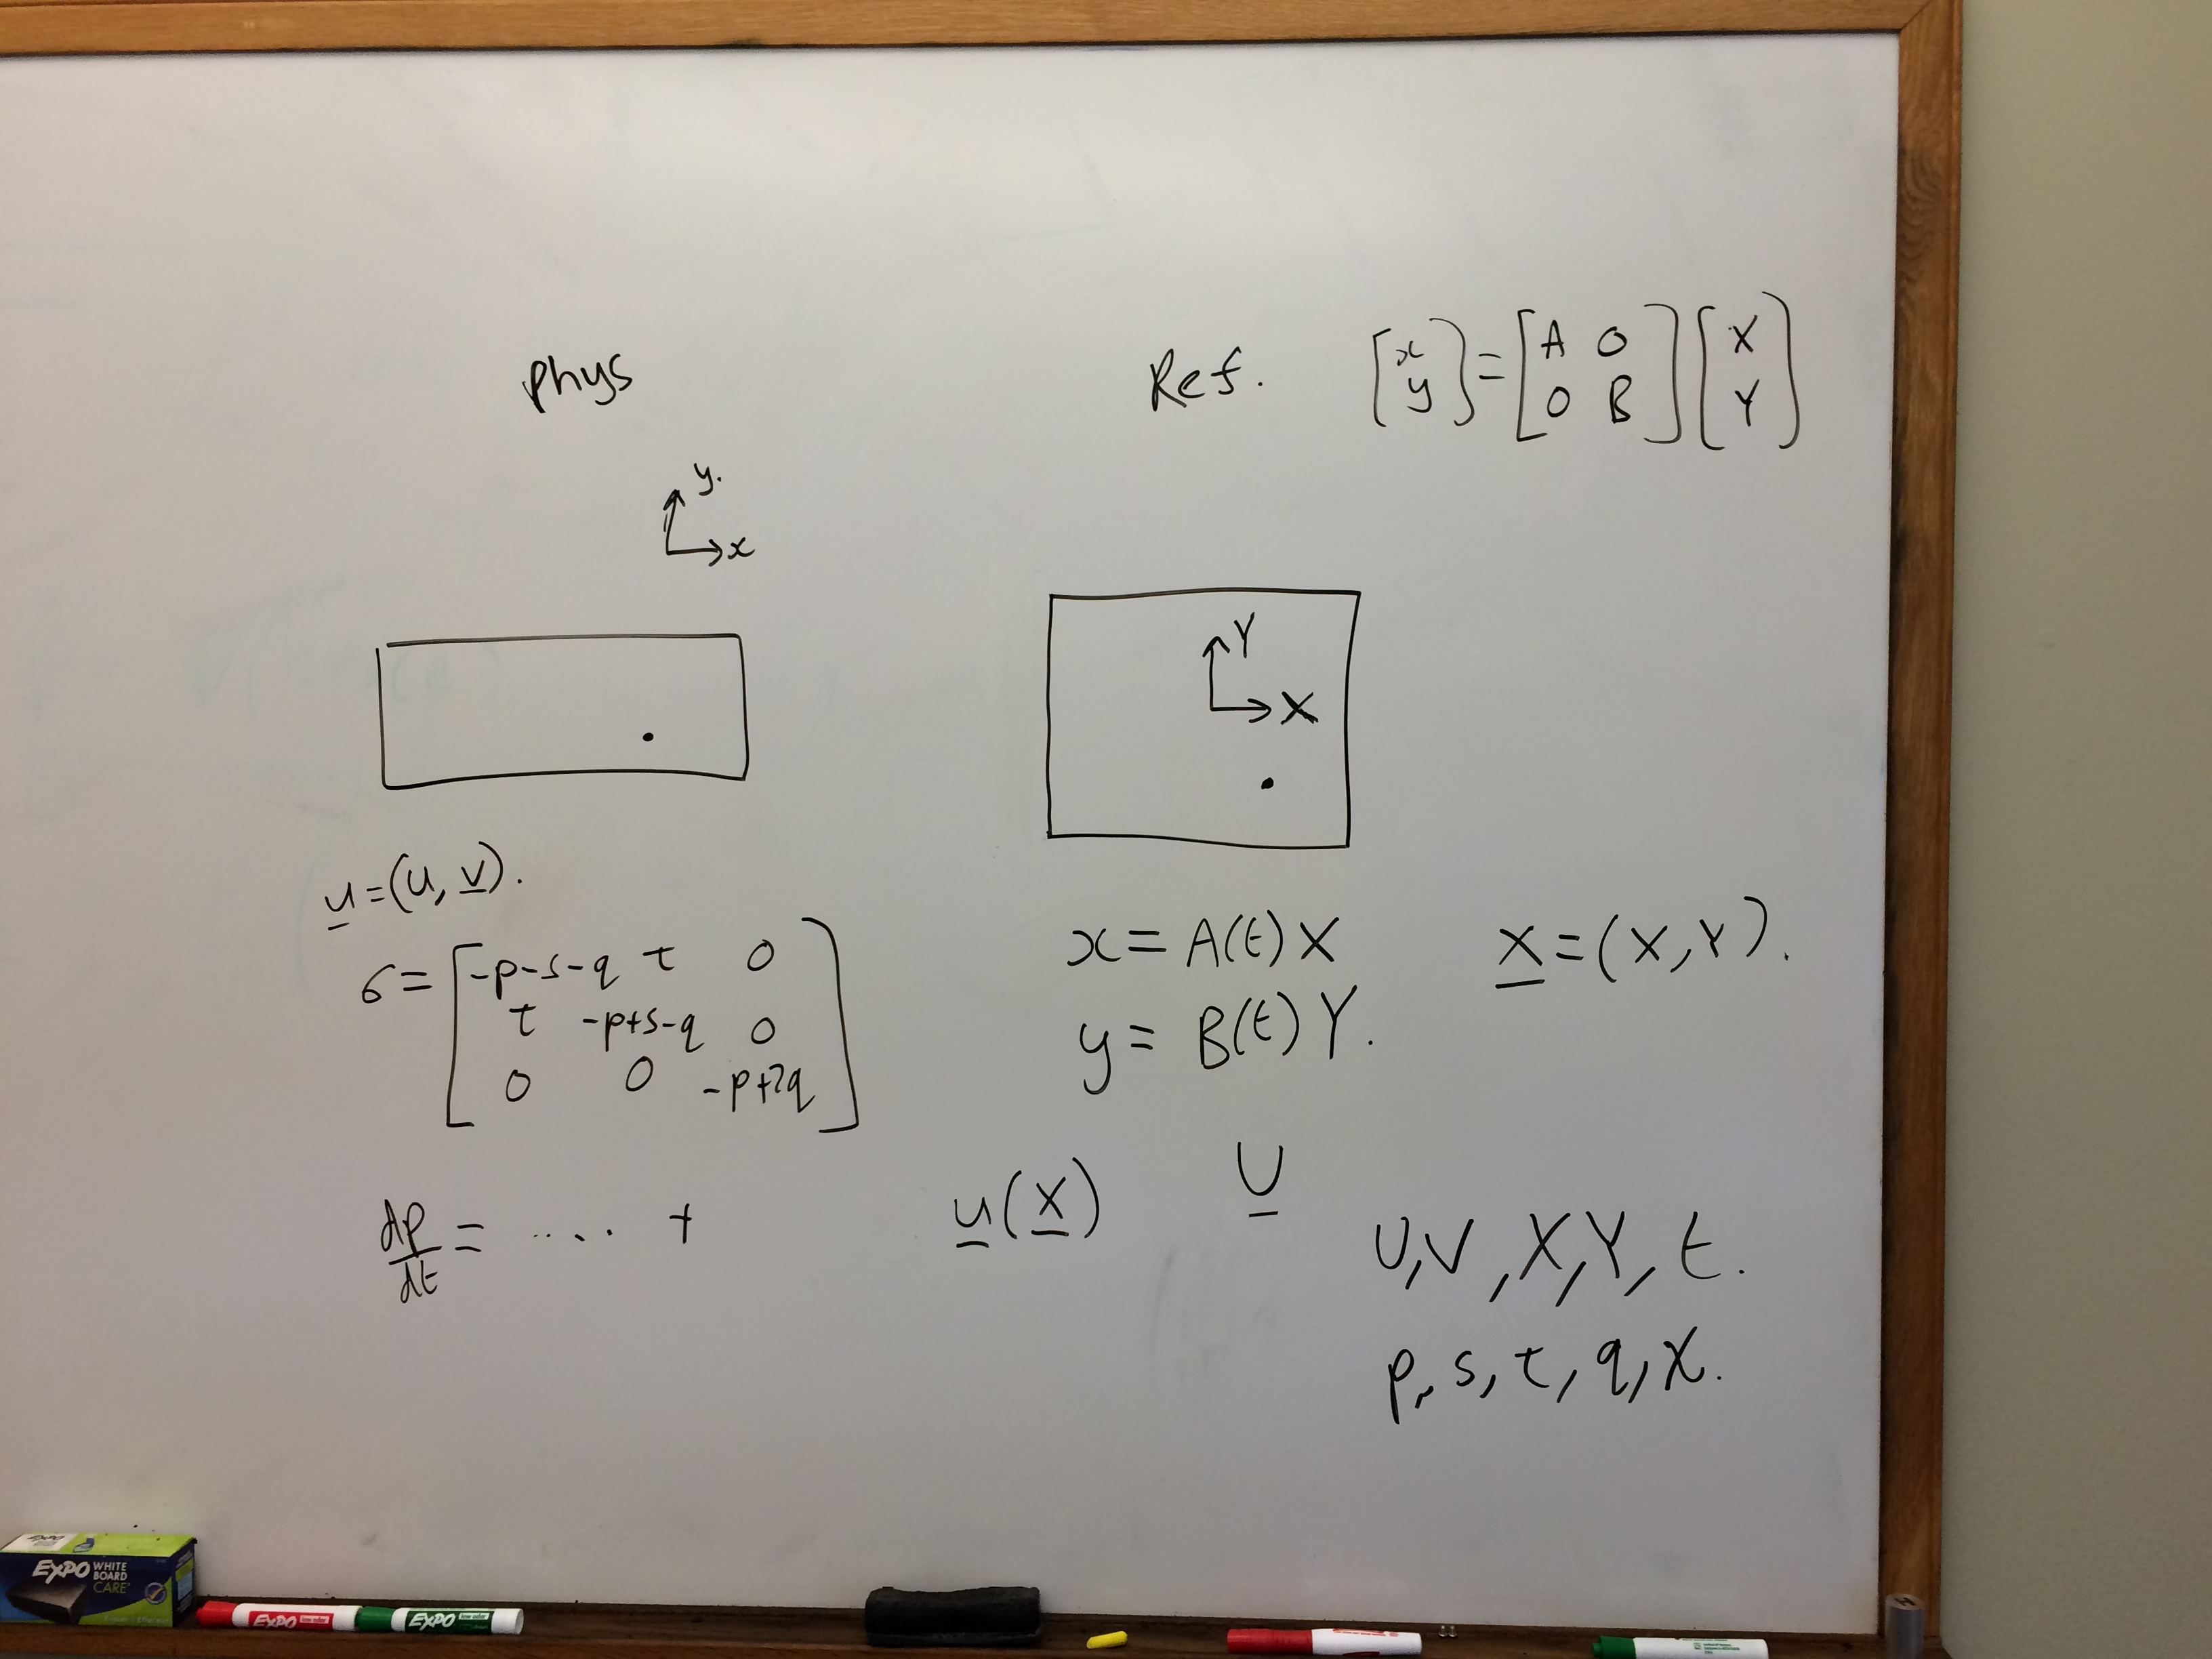
\includegraphics[width=\textwidth]{problem_1}
    \caption{Setup and graphical depiction of problem one.}
    \label{fig:prob1}
\end{figure}
Essentially, we would like to find conversions from $\nabla_\bx$ to $\nabla_\bX$, \smash{$\frac{d}{dt}_x$} to \smash{$\frac{d}{dt}_X$} (note that the time derivative changes because of the advective component) and from $(u, v)$ to $(U, V)$ where $U = \frac{d X}{dt}$ and $V = \frac{d Y}{dt}$. We will then use these conversions to rewrite the equations from the JCP article~\cite{rycroft15}.

The spatial derivatives can be converted simply using the chain rule:
\begin{align}
    \p_x &= \frac{\p X}{\p x}\p_X = A^{-1}\p_X, \\
    \p_y &= \frac{\p Y}{\p y}\p_Y =  B^{-1}\p_Y.
    \label{eqn:partials}
\end{align}
The Laplacian, which is needed to evaluate the smoothing term, is therefore given by
\begin{equation}
    \nabla_\bx^2 = A^{-2}\p_X^2 + B^{-2}\p_Y^2.
    \label{eqn:laplacian}
\end{equation}
We can now find an expression for the rescaled velocities by differentiating Eq.~\ref{eqn:coords}:
\begin{align}
    u &= \frac{dx}{dt} = \frac{\p A}{\p t} X + AU, \label{eqn:velu}\\
    v &= \frac{dy}{dt} = \frac{\p B}{\p t} Y + BV. \label{eqn:velv}
\end{align}
Lastly, we find an expression for the total time derivative, which is the most involved:
\begin{align}
    \frac{d}{dt} &= \p_t + (\bu\cdot\nabla_\bx)\\
&= \p_t + \left[ \begin{pmatrix}\strut\frac{dA}{dt}X + AU\\ \frac{dB}{dt}Y + BV\end{pmatrix}\cdot \begin{pmatrix}A^{-1}\p_X\\B^{-1}\p_Y\end{pmatrix}\right]\\
    &= \p_t + \frac{d \log A}{dt}X\p_X + U\p_X + \frac{d\log B}{dt}Y\p_Y + V\p_Y\\
&= \p_t + (\bxi + \bU) \cdot \nabla_\bX
    \label{eqn:d/dt}
\end{align}
where we have defined
\begin{equation}
    \bxi = \begin{pmatrix} (\p_t \log A)X \\ (\p_t \log B) Y\end{pmatrix}.
    \label{eqn:xi}
\end{equation}
The above calculation is a rather confusing result. When applying $\frac{d}{dt}$ to a scalar function $\phi(\bx, t)$, it is clear (as follows from the standard derivation) that the result is $\frac{d\phi}{dt} = (\p_t + \bu\cdot\nabla_\bx)\phi(\bx, t)$. Similarly, the calculation in a later section demonstrates that $\frac{d\phi(\bX, t)}{dt} = (\p_t + \bU\cdot\nabla_\bX)\phi(\bX, t)$. However, I see no error in the conversion above, and hence am not entirely sure under what situation the expression in Eq.~\ref{eqn:d/dt} is valid.

We can now apply the advective derivative to a scalar function $\phi(\bx, t) = \phi(\bT\bX, t)$, as will be necessary for the velocity and stress components, and see what result we get. Here, we have defined $\bT\bX = \bx$, i.e. in our case $\bT = \begin{pmatrix} A & 0 \\ 0 & B\end{pmatrix}$.

\begin{align}
    \frac{d}{dt}\phi(\bT\bX, t) &= \left(\frac{\p}{\p t} + \bu^\Trans\frac{\p}{\p \bx}\right)\phi(\bT\bX,t)\nonumber\\
    &= \left( \frac{\p}{\p t} + \bu^\Trans\bT^{-\Trans}\frac{\p}{\p \bX}\right)\phi(\bT\bX, t)\nonumber\\
&= \left(\frac{\p \bX}{\p t}\right)^\Trans\frac{\p}{\p \bX}\phi(\bT\bX, t) + \phi_t(\bT\bX, t) + \bu^\Trans\bT^{-\Trans}\frac{\p}{\p\bX}\phi(\bT\bX, t)\nonumber\\
    &= \phi_t(\bT\bX, t) + \left(\bu^\Trans\bT^{-\Trans} + \left(\frac{\p\bX}{\p t}\right)^\Trans\right)\frac{\p}{\p \bX}\phi(\bT\bX, t)\nonumber\\
    &= \phi_t(\bT\bX, t) + \left(\bu^\Trans\bT^{-\Trans} + \left(\frac{\p\bT^{-1}}{\p t}\bT{\bX}\right)^\Trans\right)\frac{\p}{\p \bX}\phi(\bT\bX, t)
    \label{eqn:d/dt_phi_AX}
\end{align}
This is a completely general expression, and can also be applied later for the second problem. We can now substitute for our specific case of $\bT$:
\begin{align}
    \frac{d}{dt}\phi(\bT\bX, t) = \phi_t(\bT\bX, t) + \bU^\Trans \frac{\p}{\p \bX}\phi(\bT\bX, t).
    \label{eqn:adv_deriv}
\end{align}
This expression is the result of calculating the second term in the parentheses explicitly (it turns out to be $\bxi$) and subsituting for $\bu$ using Eqs.~\ref{eqn:velu}, \ref{eqn:velv}.

Now we are in a position to rederive the equations from the JCP article. Starting with the equation for $u$,
\begin{align}
  \rho_0 \frac{d}{dt}\left(\frac{\p A}{\p t}X + A U\right) &= \frac{1}{A}\left(-\frac{\p p}{\p X} - \frac{\p q}{\p X} + \frac{\p s}{\p X} \right) + \frac{1}{B}\frac{\p \tau}{\p Y} \nonumber \\
    &\phantom{=} + \kappa\left(A^{-2}\frac{\p^2}{\p X^2} + B^{-2}\frac{\p^2}{\p Y^2}\right)\left(\frac{\p A}{\p t} X + A U\right), \label{eqn:u}\\
    \rho_0 \left(\frac{\p^2 A}{\p t^2}X + 2\frac{\p A}{\p t}U + A\frac{d U}{dt}\right) &= \frac{1}{A}\left(-\frac{\p p}{\p X} - \frac{\p q}{\p X} + \frac{\p s}{\p X} \right) + \frac{1}{B}\frac{\p \tau}{\p Y} \nonumber \\
    &\phantom{=} + \kappa\left(A^{-1}\frac{\p^2 U}{\p X^2} + B^{-2}A\frac{\p^2 U}{\p Y^2}\right).
\end{align}
We have left $\frac{d U}{dt}$ rather than expand it due to the points highlighted in the paragraph following Eq.~\ref{eqn:xi}. We can derive a very similar expression for the equation for $v$:
\begin{align}
  \rho_0 \left(\frac{\p^2 B}{\p t^2}Y + 2\frac{\p B}{\p t}V + B\frac{d V}{dt}\right) &= \frac{1}{B}\left(-\frac{\p p}{\p Y} - \frac{\p q}{\p Y} - \frac{\p s}{\p Y}\right) + \frac{1}{A}\frac{\p \tau}{\p X} \nonumber \\
    &\phantom{=} + \kappa \left(A^{-2}B\frac{\p V}{\p X^2} + B^{-1}\frac{\p V}{\p Y^2}\right). \label{eqn:v}
\end{align}
Now we can go on to derive the transformed equations for the stress components:
\begin{align}
    \frac{\p p}{\p t} + \bU\cdot\nabla_\bX p &= -K\left(A^{-1}\left[\frac{\p A}{\p t} + A\frac{\p U}{\p X}\right] + B^{-1}\left[\frac{\p B}{\p t} + B\frac{\p V}{\p Y}\right]\right)\nonumber\\
    &= -K \left(\frac{\p \log A}{\p t} + \frac{\p U}{\p X} + \frac{\p \log B}{\p t} + \frac{\p V}{\p Y}\right)\nonumber\\
    &= -K \left(\frac{\p \xi_1}{\p X} + \frac{\p U}{\p X} + \frac{\p \xi_2}{\p Y} + \frac{\p V}{\p Y}\right).
    \label{eqn:p}
\end{align}
The symmetry when written as material derivatives of $\bxi$ is suggestive; I am not sure whether it would be best to use time derivatives of $\log A$ and $\log B$ or to track $\bxi$ as its own quantity and compute reference derivatives of the components of $\bxi$. The equations for $q$ and $s$ are
\begin{align}
    \label{eqn:q}
    \frac{\p q}{\p t} + \bU\cdot \nabla_\bX q &= -\frac{\mu}{3} \left(\frac{\p \xi_1}{\p X} + \frac{\p U}{\p X} + \frac{\p \xi_2}{\p Y} + \frac{\p V}{\p Y}\right) - \frac{2\mu q \Dpl}{\bar{s}}, \\
    \label{eqn:s}
    \frac{\p s}{\p t} + \bU\cdot \nabla_\bX s &= -2\Omega\tau + \mu \left(\frac{\p \xi_1}{\p X} - \frac{\p \xi_2}{\p Y} + \frac{\p U}{\p X} - \frac{\p V}{\p Y}\right) - \frac{2\mu s \Dpl}{\bar{s}},
\end{align}
where the spin is given by
\begin{equation}
  \Omega = \frac{1}{2}\left(\frac{B}{A}\frac{\p V}{\p X} - \frac{A}{B}\frac{\p U}{\p Y}\right).
    \label{eqn:prob_1_spin}
\end{equation}
Finally, the equation for $\tau$ is
\begin{equation}
    \label{eqn:tau}
    \frac{\p \tau}{\p t} + \bU\cdot \nabla_\bX\tau = 2\Omega s + \mu\left(\frac{A}{B} \frac{\p U}{\p Y} + \frac{B}{A} \frac{\p V}{\p X}\right) - \frac{2\mu\tau \Dpl}{\bar{s}}.
\end{equation}
Note that while Eqs.~\ref{eqn:p}, \ref{eqn:q}, and \ref{eqn:s} gain additional source terms from $\bxi$, the shear stress component $\tau$ does not.

\subsection*{Quasi-static Projection}
We now consider how the quasi-static projection scheme plays into the altered coordinate frame. We need to scale time, $t\rightarrow \tilde{t}/\epsilon$, and the transformed velocity gradient, $\nabla_\bX\bU\rightarrow\epsilon\widetilde{\nabla_\bX\bU}$. First, consider the velocity gradient, $\nabla\bu$. Then,
\begin{align*}
    \nabla\bu &= \left(\bT^{-1}\nabla_\bX\right)\frac{d}{dt}\left(\bT\bX\right)\\
    &= \bT^{-1}\nabla_\bX\left(\frac{d\bT}{dt}\bX + \bT\bU\right)\\
    &= \left(\bT^{-1}\frac{d\bT}{dt} + \nabla_\bX\bU\right)
\end{align*}
and naturally we can take the transpose to get $\left(\nabla\bu\right)^\Trans$. This actually applies for any general transformation $\bT$. The time derivative of $\bu$ is
\begin{equation}
  \frac{d\bu}{dt} = \frac{d^2\left(\bT\bX\right)}{dt^2}\\
  = \frac{d}{dt}\left(\frac{d\bT}{dt}\bX + \bT\bU\right)\\
  = \frac{d^2\bT}{dt^2}\bX + 2\frac{d\bT}{dt}\bU + \bT\frac{d\bU}{dt}.
\end{equation}
Now, we can write down the equation of motion in the transformed frame as
\begin{equation}
    \left(\bT^{-T}\nabla_\bX\right)\cdot\bsig = \rho_0\left(\frac{d^2\bT}{dt^2}\bX + 2\frac{d\bT}{dt}\bU + \bT\frac{d\bU}{dt}\right)
    \label{eqn:eqn_of_motion}
\end{equation}
so that when we rescale $t\rightarrow\tilde{t}/\epsilon$, we obtain
\begin{equation}
    \left(\bT^{-T}\nabla_\bX\right)\cdot\bsig = \rho_0\left(\epsilon^2\frac{d^2\bT}{d\tilde{t}^2}\bX + 2\epsilon\frac{d\bT}{d\tilde{t}}\bU + \epsilon\bT\frac{d\bU}{d\tilde{t}}\right).
    \label{eqn:eqn_of_motion_rescaled}
\end{equation}
Dropping higher order terms in $\epsilon$, we find that
\begin{equation}
    \left(\bT^{-T}\nabla_\bX\right)\cdot\bsig = 0
  \label{eqn:quasi_static_sigma}
\end{equation}
%So that this ``modified divergence'' of the stress is zero, for any transformation $\bT$. We can rewrite this in two ways by switching to index notation. First, note that:
%\begin{align*}
    %\left(\left(\bT^{-1}\nabla_\bX\right)\cdot\bsig\right)_i &= T^{-1}_{lj}\p_j\sigma_{li}\\
    %&= \p_j(T^{-1}_{lj}\sigma_{li}) - (\p_jT^{-1}_{lj})\sigma_{li}\\
    %&= \p_j(T^{-1}_{lj}\sigma_{li}) - 0\\
    %&= \nabla_\bX \cdot (\bT^{-T}\bsig)
%\end{align*}
%So, if preferable, we can also consider the divergence of this ``modified stress'' to be zero. Last, we can derive probably the least useful equation of the three,
%\begin{align*}
    %\left(\left(\bT^{-1}\nabla_\bX\right)\cdot\bsig\right)_i &= T^{-1}_{lj}\p_j\sigma_{li}\\
    %&= T^{-T}_{jl}\p_j\sigma_{li}\\
    %&= \bT^{-T}:\left(\nabla_\bX \bsig\right)
%\end{align*}
%So that this contraction is also zero.
Now, consider the evolution equation for the components of stress:
\begin{align}
    \frac{\mcD\bsig}{\mcD t} &= \bC : \left(\bD - \bDpl\right) \nonumber \\
    &= \bC : \left( \frac{\nabla\bu + (\nabla\bu)^\Trans}{2} - \bDpl\right) \nonumber\\
    &= \bC : \left( \frac{1}{2} \left[ \bT^{-1}\frac{d\bT}{dt} + \nabla_\bX\bU + \bT^{-\Trans}\frac{d\bT^\Trans}{dt} + (\nabla_\bX\bU)^\Trans\right]  - \bDpl \right),\\
    \frac{\mcD \bsig}{\mcD \tilde{t}} &= \bC : \left( \frac{1}{2} \left[ \bT^{-1}\frac{d\bT}{d\tilde{t}} + \widetilde{\nabla_\bX\bU} + \bT^{-\Trans}\frac{d\bT^\Trans}{d\tilde{t}} + (\widetilde{\nabla_\bX\bU})^\Trans\right]  - \frac{\bDpl}{\epsilon} \right) \nonumber \\
    &= \bC : \left(\bD - \frac{\bDpl}{\epsilon}\right).
\end{align}
So again, for any arbitrary transformation, we see that at long times the plastic deformation dominates and the quasi-static scheme can be employed as usual.
Now, let's consider a formulation of the QS projection scheme. We can, as in the usual case, neglect the $\bC:\bD$ term, which leads to
\begin{equation}
  \frac{\bsig_* - \bsig_n}{\Delta t} = -\bsig_n\cdot\bOmega_n + \bOmega_n\cdot\bsig_n - \left(\bU_n\cdot\nabla_\bX\right)\bsig_n - \bC:\bDpl.
  \label{eqn:qs_first_step}
\end{equation}
In Eq.~\ref{eqn:qs_first_step}, $\bOmega$ is given by Eq.~\ref{eqn:prob_1_spin}. Naturally, for the Truesdell rate, the right hand side would look slightly different. Note that this is identical to the untransformed case, except for modifications to the spin term. In the implementation, the advective derivative will remain the same and the contraction will remain the same. Then, if we have the velocity $\mathbf{v}_{n+1}$, we can calculate the rate of deformation tensor $\bD_{n+1}$, and the stress at the next timestep is given by:
\begin{equation}
    \frac{\bsig_{n+1} - \bsig_*}{\Delta t} = \bC : \bD_{n+1}
    \label{eqn:qs_second_step}
\end{equation}
An important point as that the $\bD_{n+1}$ appearing above is the \emph{untransformed} velocity. If we multiply by sides by $\bT^{-T}$ and take the divergence, using that $\nabla_\bX\cdot(\bT^{-T}\bsig_{n+1})=0$, we find that:
\begin{equation}
    \nabla_\bX\cdot(\bT^{-T}\bsig_*) = -\Delta t \nabla_\bX\cdot\left(\bT^{-T}\bC:\bD_{n+1}\right)
\end{equation}
Alternatively, we can take the ``modified divergence'':
\begin{equation}
    \left(\bT^{-T}\nabla_\bX\right)\cdot \bsig_* = -\Delta t\left(\bT^{-T}\nabla_\bX\right)\cdot\bC:\bD_{n+1}
    \label{eqn:mg_eqn}
\end{equation}
Which is another valid way to write down the relation. It seems that this is the easiest way to go about it, as it simply introduces factors of $A^{-1}$ and $B^{-1}$ into some derivatives in the code.

Now, let's consider expanding Eq.~\ref{eqn:qs_second_step} componentwise. It is simple enough to show (and thus will not be shown here) that:
\begin{equation*}
    (\bC : \bD)_{ij} = \lambda \left(\p_k v_k\right)\delta_{ij} + \mu\left(\p_i v_j + \p_j v_i\right) \end{equation*}
    We use Einstein summation notation above and $\p_k$, $v_k$ are both the untransformed coordinates. We would like to write the componentwise equation in terms of the transformed velocities and transformed spatial derivatives. Let $d_i$ denote the partial derivative with respect to $X_i$ (i.e., the $i^{th}$ transformed spatial coordinate). This applies for any non spatially-varying, but time-dependent transformation $\bT(t)$. Then we can write, first transforming the derivatives and then the velocities:
\begin{align}
    \left(\bC : \bD\right)_{ij} &= \lambda \left(T^{-T}_{kl}d_lv_k\right)\delta_{ij} + \mu\left(T^{-T}_{il}d_lv_j + T^{-T}_{jl}d_lv_i\right)\nonumber\\
    &= \lambda \left( T^{-T}_{kl}d_l \left[\frac{\p T_{kq}}{\p t}X_q + T_{kq} U_q\right]\right)\delta_{ij}+ \mu \left(T^{-T}_{il}d_l\left[\frac{\p T_{jq}}{\p t}X_q + T_{jq}U_q\right] + T^{-T}_{jl}d_l\left[\frac{\p T_{iq}}{\p t}X_q + T_{iq}U_q\right]\right)\nonumber\\
    &= \lambda \left(T^{-T}_{kl}\frac{\p T_{kq}}{\p t}\delta_{lq} + T^{-T}_{kl}T_{kq}d_lU_q \right)\delta_{ij} + \mu \left(T^{-T}_{il}\frac{\p T_{jq}}{\p t}\delta_{lq} + T^{-T}_{il}T_{jq}d_lU_q + T^{-T}_{jl}\frac{\p T_{iq}}{\p t}\delta_{lq} + T^{-T}_{jl}T_{iq}d_lU_q\right)\nonumber\\
    &= \lambda \left(T^{-T}_{kl} \frac{\p T_{kl}}{\p t} + T_{kq}T^{-T}_{kl}d_lU_q\right)\delta_{ij} + \mu \left(T^{-T}_{il}\frac{\p T_{jl}}{\p t} + T_{jq}T^{-T}_{il}d_lU_q + T^{-T}_{jl}\frac{\p T_{il}}{\p t} + T_{iq}T^{-T}_{jl}d_lU_q \right) \nonumber\\
    &= \lambda \left(T^{-1}_{lk} \frac{\p T_{kl}}{\p t} + d_lU_l\right)\delta_{ij} + \mu \left(T^{-1}_{li}\frac{\p T_{jl}}{\p t} + T_{jq}T^{-1}_{li}d_lU_q + T^{-1}_{lj}\frac{\p T_{il}}{\p t} + T_{iq}T^{-1}_{lj}d_lU_q \right)
    \label{eqn:c_contr_d}
\end{align}
This is a pretty beastly equation, and it does not seem easy to re-interpret into matrix form. We can, however, simply look at the componentwise expressions:
\begin{align*}
    (\bC : \bD)_{11} &= \lambda\left(\frac{\p \log A}{\p t} + \frac{\p \log B}{\p t} + \boldsymbol{\nabla}_X\cdot\bU\right) + 2\mu\left(\frac{\p \log A}{\p t} + \frac{\p U}{\p X}\right)\\
    (\bC : \bD)_{12} &= \mu\left(\frac{B}{A}\frac{\p V}{\p X} + \frac{A}{B}\frac{\p U}{\p Y}\right) = (\bC : \bD)_{21}\\
    (\bC : \bD)_{22} &= \lambda \left(\frac{\p \log A}{\p t} + \frac{\p \log B}{\p t} + \boldsymbol{\nabla}_X\cdot\bU\right) + 2\mu\left(\frac{\p \log B}{\p t} + \frac{\p V}{\p Y}\right)\\
    (\bC : \bD)_{33} &= \lambda\left(\frac{\p \log A}{\p t} + \frac{\p \log B}{\p t} + \boldsymbol{\nabla}_X\cdot \mathbf{U}\right)\\
    (\bC : \bD)_{13} &= (\bC : \bD)_{23} = (\bC : \bD)_{31} = (\bC : \bD)_{32} = 0
\end{align*}
These expressions will be necessary for the ``correction step'' where we obtain $\bsig_{n+1}$ from $\bsig_*$. Eq.~\ref{eqn:c_contr_d} is necessary for the projection step, and we will now take the ``modified divergence'' of it. First, consider the $\lambda$ component of Eq.~\ref{eqn:c_contr_d}.
\begin{align*}
    \left[\bT^{-T}\boldsymbol{\nabla}_X\cdot(\bC:\bD)_\lambda\right]_i &= \lambda T^{-1}_{nm}d_n\left(T^{-1}_{lk}\frac{\p T_{lk}}{\p t} + d_lU_l\right)\delta_{mi}\\
    &= \lambda T^{-1}_{nm}d_nd_lU_l\delta_{mi}
\end{align*}
Note that, in the above equation, we have assumed $\bT = \bT(t)$ is spatially homogeneous. A spatially-varying transform would gain some additional terms from the application of the product rule. Now, we can consider the $\mu$ component, dropping the terms not proportional to $U$ as $\bT$ has no spatial dependence,
\begin{align}
    \left[\bT^{-T}\boldsymbol{\nabla}_X\cdot(\bC:\bD)_\mu\right]_i &= \left(T^{-1}_{nm}d_n\right)\mu\left(T_{iq}T^{-1}_{lm}d_l U_q + T_{mq}T^{-1}_{lio}d_lU_q\right)\nonumber\\
    &= \mu\left(T^{-1}_{nm}T_{iq}T^{-1}_{lm}d_nd_lU_q + T^{-1}_{nm}T_{mq}T^{-1}_{li}d_nd_lU_q\right)\nonumber\\
    &= \mu\left(T^{-1}_{nm}T_{iq}T^{-1}_{lm}d_nd_lU_q + T^{-1}_{li}d_ld_qU_q\right)
    \label{eqn:divCD}
\end{align}
We can now write these out componentwise:
\begin{align*}
    \left[\bT^{-T}\boldsymbol{\nabla}_X\cdot(\bC:\bD)\right]_1 &= \frac{\lambda}{A}\left(\frac{\p^2 U}{\p X^2} + \frac{\p^2 V}{\p X\p Y}\right) + \mu\left(\frac{2}{A}\frac{\p^2 U}{\p X^2} + \frac{A}{B^2}\frac{\p^2 U}{\p Y^2} + \frac{1}{A}\frac{\p^2 V}{\p X\p Y}\right)\\
    \left[\bT^{-T}\boldsymbol{\nabla}_X\cdot(\bC:\bD)\right]_2 &= \frac{\lambda}{B}\left(\frac{\p^2 U}{\p X \p Y} + \frac{\p^2 V}{\p Y^2}\right) + \mu\left(\frac{2}{B}\frac{\p^2 V}{\p Y^2} + \frac{B}{A^2}\frac{\p^2 V}{\p X^2} + \frac{1}{B}\frac{\p^2 U}{\p X\p Y}\right)
\end{align*}
Now we can also easily transform the two components of the source term:
\begin{align*}
    \left(\bT^{-1}\boldsymbol{\nabla}_X\cdot\bsig_*\right)_1 &= \frac{1}{A}\left(-\frac{\p p_*}{\p X} - \frac{\p q_*}{\p X} + \frac{\p s_*}{\p X}\right) + \frac{1}{B}\frac{\p \tau_*}{\p Y}\\
\left(\bT^{-1}\boldsymbol{\nabla}_X\cdot\bsig_*\right)_2 &= \frac{1}{B}\left(-\frac{\p p_*}{\p Y} - \frac{\p q_*}{\p Y} - \frac{\p s_*}{\p Y}\right)  + \frac{1}{A}\frac{\p \tau_*}{\p X}
\end{align*}
So that we can put these all together and write down the multigrid system of equations:
\begin{align*}
    \frac{\lambda}{A}\left(\frac{\p^2 U}{\p X^2} + \frac{\p^2 V}{\p X\p Y}\right) + \mu\left(\frac{2}{A}\frac{\p^2 U}{\p X^2} + \frac{A}{B^2}\frac{\p^2 U}{\p Y^2} + \frac{1}{A}\frac{\p^2 V}{\p X\p Y}\right) &= \frac{1}{A\Delta t}\left(\frac{\p p_*}{\p X} + \frac{\p q_*}{\p X} - \frac{\p s_*}{\p X}\right) - \frac{1}{B\Delta t}\frac{\p \tau_*}{\p Y}\\
    \frac{\lambda}{B}\left(\frac{\p^2 U}{\p X \p Y} + \frac{\p^2 V}{\p Y^2}\right) + \mu\left(\frac{2}{B}\frac{\p^2 V}{\p Y^2} + \frac{B}{A^2}\frac{\p^2 V}{\p X^2} + \frac{1}{B}\frac{\p^2 U}{\p X\p Y}\right) &= \frac{1}{B\Delta t}\left(\frac{\p p_*}{\p Y} + \frac{\p q_*}{\p Y} + \frac{\p s_*}{\p Y}\right) - \frac{1}{A\Delta t}\frac{\p \tau_*}{\p X}.
\end{align*}
Or, regrouping these terms,
\begin{align*}
    \frac{\lambda + 2\mu}{A}\frac{\p^2 U}{\p X^2} + \frac{\lambda + \mu}{A}\frac{\p^2 V}{\p X\p Y} + \frac{\mu A}{B^2}\frac{\p^2 U}{\p Y^2} &= \frac{1}{A\Delta t}\left(\frac{\p p_*}{\p X} + \frac{\p q_*}{\p X} - \frac{\p s_*}{\p X}\right) - \frac{1}{B\Delta t}\frac{\p \tau_*}{\p Y}\\
    \frac{\lambda + 2\mu}{B}\frac{\p^2 V}{\p Y^2} + \frac{\lambda + \mu}{B}\frac{\p^2 U}{\p X\p Y} + \frac{\mu B}{A^2}\frac{\p^2 V}{\p X^2} &= \frac{1}{B\Delta t}\left(\frac{\p p_*}{\p Y} + \frac{\p q_*}{\p Y} + \frac{\p s_*}{\p Y}\right) - \frac{1}{A\Delta t}\frac{\p \tau_*}{\p X}.
\end{align*}
And now, using that $\lambda = K - \frac{2}{3}\mu$ where $K$ is the bulk modulus, we can write that $\lambda + \mu = K + \frac{1}{3}\mu = K'$, and that $\lambda + 2\mu = K + \frac{4}{3}\mu = K' + \mu$. Then,
\begin{align*}
    \frac{K' + \mu}{A}\frac{\p^2 U}{\p X^2} + \frac{K'}{A}\frac{\p^2 V}{\p X\p Y} + \frac{\mu A}{B^2}\frac{\p^2 U}{\p Y^2} &= \frac{1}{A\Delta t}\left(\frac{\p p_*}{\p X} + \frac{\p q_*}{\p X} - \frac{\p s_*}{\p X}\right) - \frac{1}{B\Delta t}\frac{\p \tau_*}{\p Y}\\
    \frac{K' + \mu}{B}\frac{\p^2 V}{\p Y^2} + \frac{K'}{B}\frac{\p^2 U}{\p X\p Y} + \frac{\mu B}{A^2}\frac{\p^2 V}{\p X^2} &= \frac{1}{B\Delta t}\left(\frac{\p p_*}{\p Y} + \frac{\p q_*}{\p Y} + \frac{\p s_*}{\p Y}\right) - \frac{1}{A\Delta t}\frac{\p \tau_*}{\p X}.
\end{align*}
And now if we add in the viscosity terms, where $\kappa$ is the viscosity parameter and $\kappa' := \frac{\kappa}{\Delta t}$, we then have:
\begin{align}
    \frac{K' + \mu + \kappa'}{A}\frac{\p^2 U}{\p X^2} + \frac{K'}{A}\frac{\p^2 V}{\p X\p Y} + \frac{(\mu + \kappa') A}{B^2}\frac{\p^2 U}{\p Y^2} &= \frac{1}{A\Delta t}\left(\frac{\p p_*}{\p X} + \frac{\p q_*}{\p X} - \frac{\p s_*}{\p X}\right) - \frac{1}{B\Delta t}\frac{\p \tau_*}{\p Y}\\
    \frac{K' + \mu + \kappa'}{B}\frac{\p^2 V}{\p Y^2} + \frac{K'}{B}\frac{\p^2 U}{\p X\p Y} + \frac{(\mu + \kappa') B}{A^2}\frac{\p^2 V}{\p X^2} &= \frac{1}{B\Delta t}\left(\frac{\p p_*}{\p Y} + \frac{\p q_*}{\p Y} + \frac{\p s_*}{\p Y}\right) - \frac{1}{A\Delta t}\frac{\p \tau_*}{\p X}.
    \label{eqn:mg_system}
\end{align}
Which is our ultimate system of equations for the multigrid solver, with the source terms appearing on the right hand side. Note that this is precisely what one would obtain by transforming Eqs. $57$ and $58$ in \cite{rycroft15} directly; this, unfortunately, would have been a much simpler way to obtain the result without all the tensor-induced pain and suffering that has been demonstrated above.

Now that we have these equations derived, let's write out the quasi-static projection scheme explicitly. We first have:
\begin{align}
    \frac{p_* - p_n}{\Delta t} &= -\advn p_n\\
    \frac{q_* - q_n}{\Delta t} &= -\advn q_n - \frac{2\mu\widetilde{\Dpl}_nq_n}{\bar{s}_n}\\
    \frac{s_* - s_n}{\Delta t} &= -\advn s_n - 2\Omega_n\tau_n - \frac{2\mu\widetilde{\Dpl}_ns_n}{\bar{s}_n}\\
    \frac{\tau_* - \tau_n}{\Delta t} &= -\advn \tau_n + 2\Omega_n s_n - \frac{2\mu\widetilde{\Dpl}_n\tau_n}{\bar{s}_n}
    \label{eqn:adv_step}
\end{align}

Which are the componentwise equations for the intermediate stress $\bsig_*$. If the velocity at the next timestep $\bU_{n+1}$ is known, then we can calculate:
\begin{align}
    \frac{p_{n+1}-p_*}{\Delta t} &= -K\left(\frac{\p U_n}{\p X} + \frac{\p V_n}{\p Y} + A^{-1}\frac{\p A}{\p t} + B^{-1}\frac{\p B}{\p t}\right)\\
    \frac{q_{n+1}-q_*}{\Delta t} &= -\frac{\mu}{3}\left(\frac{\p U_n}{\p X} + \frac{\p V_n}{\p Y} + A^{-1}\frac{\p A}{\p t} + B^{-1}\frac{\p B}{\p t}\right)\\
    \frac{s_{n+1}-s_*}{\Delta t} &= \mu\left(\frac{\p U_n}{\p X} - \frac{\p V_n}{\p Y} + A^{-1}\frac{\p A}{\p t} - B^{-1}\frac{\p B}{\p t}\right)\\
    \frac{\tau_{n+1}-\tau_*}{\Delta t} &= \mu\left(\frac{A}{B}\frac{\p U_n}{\p Y} + \frac{B}{A}\frac{\p V_n}{\p X} \right)
    \label{eqn:proj_step}
\end{align}
To find $\bU_{n+1}$, we solve Eqs.~\ref{eqn:mg_system}.
\section*{Problem 2(a) -- Simple Shear}
Let us now consider a simplified version of the second problem: simple shear. In this case, we have
\begin{align}
    x(t) &= X + \lambda t Y, \label{eqn:sshear_x} \\
    y(t) &= Y \label{eqn:sshear_y}
\end{align}
and hence the corresponding transformation is
\begin{equation}
    \bT = \begin{pmatrix} 1 & \lambda t \\ 0 & 1 \end{pmatrix}.
\end{equation}
Using the chain rule as before, the spatial derivatives in the physical
coordinates are given by
\begin{align}
    \p_x &= \p_X, \label{eqn:sshear_d/dx} \\
    \p_y &= \frac{\p X}{\p y}\p_X + \frac{\p Y}{\p y}\p_Y = \p_Y - \lambda t \p_X,
    \label{eqn:sshear_d/dy}
\end{align}
and the Laplacian satisfies
\begin{equation}
    \nabla_\bx^2 = \nabla_\bX^2 + \lambda^2t^2\p_X^2 - 2\lambda t\p_Y\p_X.
    \label{eqn:sshear_lapl}
\end{equation}
The transformed velocity components are given by
\begin{align}
    u &= \frac{dx}{dt} = U + \lambda (Y + tV), \label{eqn:sshear_u}\\
    v &= \frac{dy}{dt} = V. \label{eqn:sshear_v}
\end{align}
The two terms in Eq.~\ref{eqn:sshear_u} are physically reasonable. The $\lambda Y$ term is due to the motion of the transformed coordinate system with respect to the physical coordinate system. The $\lambda t V$ term occurs because a vertical velocity in the transformed system has a horizontal component in the physical system.

Now, we can use Eq.~\ref{eqn:adv_deriv} to calculate the advective time derivative of a field for this transformation. First, we can calculate some useful quantities that appear in the formula:
\begin{equation}
    \bT = \begin{pmatrix} 1 & \lambda t \\ 0 & 1 \end{pmatrix}, \qquad
    \bT^\Trans = \begin{pmatrix} 1 & 0 \\ \lambda t & 1 \end{pmatrix}, \qquad
    \bT^{-1} = \begin{pmatrix} 1 & -\lambda t \\ 0 & 1 \end{pmatrix}, \qquad
    \bT^{-\Trans} = \begin{pmatrix} 1 & 0 \\ -\lambda t & 1 \end{pmatrix}.
\end{equation}
Hence
\begin{equation}
\frac{\p \bT^{-1}}{\p t} = \begin{pmatrix} 0 & -\lambda \\ 0 & 0 \end{pmatrix}, \qquad
\bu^\Trans\bT^{-\Trans} = \begin{pmatrix} u - \lambda t v \\ v \end{pmatrix}^\Trans
=  \begin{pmatrix} U + \lambda Y \\ V \end{pmatrix}^\Trans.
\end{equation}
and therefore
\begin{equation}
\left(\frac{\p \bT^{-1}}{\p t}\bT\bX\right)^\Trans = \left[\begin{pmatrix} 0 & -\lambda \\ 0 & 0 \end{pmatrix}
\begin{pmatrix} 1 & \lambda t \\ 0 & 1 \end{pmatrix} \begin{pmatrix} X \\ Y \end{pmatrix} \right]^\Trans\\
= \begin{pmatrix} -\lambda Y \\ 0 \end{pmatrix}^\Trans.
\end{equation}
Plugging these all in to Eq.~\ref{eqn:adv_deriv}, we find that for some arbitrary scalar function $\phi(\bT\bX, t)$,
\begin{equation}
\frac{d\phi(\bT\bX)}{dt} = \phi_t + \left[ \begin{pmatrix}U + \lambda Y\\ V \end{pmatrix}^\Trans - \begin{pmatrix}\lambda Y \\ 0\end{pmatrix}^\Trans\right]\frac{\p\phi}{\p \bX}\nonumber\\
    = \phi_t + (\bU\cdot\nabla_\bX)\phi.
    \label{eqn:sshear_adv_deriv}
\end{equation}
Equation~\ref{eqn:sshear_adv_deriv} again demonstrates that only the transformed velocity is needed for advection in the transformed frame. It is potentially possible to show this directly from Eq.~\ref{eqn:adv_deriv}.

We can now transform the equations from the JCP article:
\begin{align}
    \rho_0 \frac{d}{dt}\left(U + \lambda[Y + tV]\right) &= -\frac{\p p}{\p X} - \frac{\p q}{\p X} + \frac{\p s}{\p X} + \frac{\p \tau}{\p Y} - \lambda t \frac{\p \tau}{\p X} \nonumber\\
    &\phantom{=} + \kappa\left(\nabla_\bX^2 + \lambda^2t^2\frac{\p^2}{\p X^2} - 2\lambda t \frac{\p^2}{\p X\p Y}\right)\left(U + \lambda[Y + tV]\right),\nonumber\\
    \rho_0\left(\frac{d}{dt}(U + \lambda t V) + \lambda V\right) &= -\frac{\p p}{\p X} - \frac{\p q}{\p X} + \frac{\p s}{\p X} - \lambda t\frac{\p \tau}{\p X} \nonumber \\
    &\phantom{=} + \kappa\left(\nabla_\bX^2 + \lambda^2t^2\frac{\p^2}{\p X^2} - 2\lambda t \frac{\p^2}{\p X\p Y}\right)(U + \lambda t V). \label{eqn:sshear_u_evol}
\end{align}
The quantity $U + \lambda t V$ appears on both sides in Eq.~\ref{eqn:sshear_u_evol}; this is perhaps because a similar expression shows up in Eq.~\ref{eqn:sshear_u}, but it might also be a useful quantity in its own right.
The equation for $V$ is a bit simpler:
\begin{align}
    \rho_0 \frac{dV}{dt} &= -\frac{\p p}{\p Y} + \lambda t \frac{\p p}{\p X} - \frac{\p q}{\p Y} + \lambda t \frac{\p q}{\p X} - \frac{\p s}{\p Y} + \lambda t\frac{\p s}{\p X} + \frac{\p\tau}{\p X} \nonumber \\
    &\phantom{=} + \kappa \left(\nabla_\bX^2 + \lambda^2t^2\frac{\p^2}{\p X^2} - 2\lambda t\frac{\p^2}{\p X\p Y}\right) V.
    \label{eqn:sshear_v_evol}
\end{align}
Lastly, we calculate the equations for the components of stress. The equation for the pressure is
\begin{equation}
    \frac{dp}{dt} = -K\left(\frac{\p U}{\p X} + \frac{\p V}{\p Y}\right).
    \label{eqn:sshear_p_evol}
\end{equation}
It is interesting that the quantity \smash{$\frac{\p u}{\p x} + \frac{\p v}{\p y}$} is invariant under this transformation; as we will see later, \smash{$\frac{\p u}{\p y} - \frac{\p v}{\p x}$} is not, which likely says something about the fact that the transformation has a spin. The equation for $q$ component of stress is
\begin{equation}
    \frac{dq}{dt} = -\frac{\mu}{3}\left(\frac{\p U}{\p X} + \frac{\p V}{\p Y}\right) - \frac{2\mu q\Dpl}{\bar{s}}.
    \label{eqn:sshear_q_evol}
\end{equation}
The remaining two stress components require consideration of the spin, which in physical coordinates is given by
\begin{equation}
    \omega = \frac{1}{2}\left(\frac{\p v}{\p x} - \frac{\p u}{\p y}\right).
\end{equation}
Substituting in the expressions in Eqs.~\ref{eqn:sshear_d/dx},
\ref{eqn:sshear_d/dy}, \ref{eqn:sshear_u}, and \ref{eqn:sshear_v} yields
\begin{align}
    \omega &= \frac{1}{2} \left( \p_X V - (\p_Y - \lambda t \p_X) (U+\lambda Y+\lambda t V) \right) \nonumber \\
    &= \frac{1}{2} \left( \frac{\p V}{\p X} - \frac{\p U}{\p Y} + \lambda t \frac{\p U}{\p X}
    -\lambda - \lambda t \frac{\p V}{\p Y} + \lambda^2 t^2 \frac{\p V}{\p X}\right). \label{eqn:sshear_spin}
\end{align}
The first two terms in Eq.~\ref{eqn:sshear_spin} match the usual definition of
spin in an untransformed frame. The single $\lambda$ term is also reasonable,
since if $U=V=0$ then the spin will be constant. However, the other terms do
not appear to have an obvious simplification. Using Eq.~\ref{eqn:sshear_spin},
the equations for the remaining two stress components are
\begin{equation}
    \frac{ds}{dt} = -2\omega \tau + \mu\left(\frac{\p}{\p X}(U + \lambda t V) + \lambda t \frac{\p V}{\p X} - \frac{\p V}{\p Y}\right) - \frac{2\mu s \Dpl}{\bar{s}}
    \label{eqn:sshear_s_evol}
\end{equation}
and
\begin{equation}
    \frac{d\tau}{dt} = 2\omega s +\mu\left(\frac{\p}{\p Y}(U + \lambda t V) + \lambda  - \lambda t \frac{\p}{\p X}(U + \lambda t V) + \frac{\p V}{\p X}\right) - \frac{2\mu\tau\Dpl}{\bar{s}}.
    \label{eqn:sshear_tau_evol}
\end{equation}
Note the repeated occurrences of the term $U+\lambda t V$ in Eqs.~\ref{eqn:sshear_spin}, \ref{eqn:sshear_s_evol}, and \ref{eqn:sshear_tau_evol}, which could be grouped together as a possible simplification.

\section*{Truesdell Rate}
In this section, we will first derive the un-transformed equations of motion using the full Truesdell rate, and then transform them to the new variables. From there, we will attempt to deduce a good choice of transformed stres variables. We start with the funcdamental equation:
\begin{equation}
    \dot{\bsig} = \bC : \bDel
    \label{eqn:sigma_evol}
\end{equation}
where the Truesdell rate is given by:
\begin{equation}
    \dot{\bsig} = \frac{d\bsig}{dt} - \bL\cdot\bsig - \bsig\cdot\bL^\Trans + Tr(\bL)\bsig
    \label{eqn:truesdell_rate}
\end{equation}
Carrying out this contraction and solving for the material time derivative of sigma leads to the componentwise equations:
\begin{align}
    \frac{dp}{dt} &= \frac{2s}{3}\left(\frac{\p v}{\p y} - \frac{\p u}{\p x}\right) - \frac{2\tau}{3}\left(\frac{\p v}{\p x} + \frac{\p u}{\p y}\right) - \frac{1}{3}\left(3 l + p - 2q + 2\mu\right)\left(\frac{\p u}{\p x} + \frac{\p v}{\p y}\right)\\
    \frac{dq}{dt} &= \frac{1}{3}\left(p - 2q - \mu\right)\left(\frac{\p v}{\p y} + \frac{\p u}{\p x}\right) + \frac{s}{3}\left(\frac{\p v}{\p y} - \frac{\p u}{\p x}\right) - \frac{\tau}{3}\left(\frac{\p v}{\p x} + \frac{\p u }{\p y}\right) - \frac{2\mu D^{pl}}{\bar{s}}q\\
    \frac{ds}{dt} &= -2\omega\tau - \frac{2\mu\Dpl}{\bar{s}}s + \left(p + q - \mu\right)\left(\frac{\p v}{\p y} - \frac{\p u}{\p x}\right)\\
    \frac{d\tau}{dt} &= \left(\mu - p - q\right)\left(\frac{\p u}{\p y} + \frac{\p v}{\p x}\right) + 2\omega s - \frac{2\mu\Dpl}{\bar{s}}\tau.
\end{align}
In the equation for $p$, $l$ is the Lame parameter usually denoted by $\lambda$. We use $l$ to avoid confusion with the shear parameter $\lambda$. If we now transform these equations so that they are written in terms of $U, V, X, Y$, we find that:
\begin{align}
    \frac{dp}{dt} &= \frac{2s}{3}\left(\frac{\p V}{\p Y} - 2\lambda t \frac{\p V}{\p X} - \frac{\p U}{\p X}\right) - \frac{2\tau}{3}\left(\frac{\p V}{\p X} + \frac{\p U}{\p Y} + \lambda + \lambda t\left[\frac{\p V}{\p Y} - \frac{\p U}{\p X}\right] - \lambda^2t^2\frac{\p V}{\p X}\right)\nonumber\\
    &\qquad\qquad\qquad - \frac{1}{3}(3l + p - 2q + 2\mu)\left(\frac{\p U}{\p X} + \frac{\p V}{\p Y}\right)\\
    \frac{dq}{dt} &= \frac{1}{3}\left(p - 2q - \mu\right)\left(\frac{\p V}{\p Y} + \frac{\p U}{\p X}\right) + \frac{s}{3}\left(\frac{\p V}{\p Y} - 2\lambda t \frac{\p V}{\p X} - \frac{\p U}{\p X}\right) \nonumber\\
    &\qquad\qquad\qquad - \frac{\tau}{3}\left(\frac{\p V}{\p X} + \frac{\p U}{\p Y} + \lambda + \lambda t\left[\frac{\p V}{\p Y} - \frac{\p U}{\p X}\right] - \lambda^2t^2 \frac{\p V}{\p X}\right) - \frac{2\mu\Dpl}{\bar{s}}q\\
    \frac{ds}{dt} &= -\left(\frac{\p V}{\p X} - \frac{\p U}{\p Y} - \lambda - \lambda t \frac{\p V}{\p Y} + \lambda t \frac{\p U}{\p X} + \lambda^2 t^2 \frac{\p V}{\p X}\right)\tau - \frac{2\mu \Dpl}{\bar{s}}s \nonumber\\
    &\qquad\qquad\qquad + (p + q - \mu)\left(\frac{\p V}{\p Y} - 2\lambda t \frac{\p V}{\p X} - \frac{\p U}{\p X}\right)\\
    \frac{d\tau}{dt} &= (\mu - p - q)\left(\frac{\p V}{\p X} + \frac{\p U}{\p Y} + \lambda + \lambda t\left[\frac{\p V}{\p Y} - \frac{\p U}{\p X}\right] - \lambda^2t^2 \frac{\p V}{\p X}\right) \nonumber\\
    &\qquad\qquad\qquad\qquad + \left(\frac{\p V}{\p X} - \frac{\p U}{\p Y} - \lambda - \lambda t \frac{\p V}{\p Y} + \lambda t \frac{\p U}{\p X} + \lambda^2 t^2 \frac{\p V}{\p X}\right)s - \frac{2\mu\Dpl}{\bar{s}}\tau
\end{align}
If we now apply the contravariant pullback to $\bsig$, i.e., $\bsig' = T^{-1}\bsig T^{-\Trans}$, we find the following for the transformed components of the stress tensor:
\begin{align}
    p' &= p + \frac{2\lambda t}{3}\tau + \frac{\lambda^2 t^2}{3}\left(p + q + s\right)\\
    q' &= q + \frac{\lambda t}{3}\tau + \frac{\lambda^2 t^2}{6}\left(p + q + s\right)\\
    s' &= s - \lambda t \tau - \frac{\lambda^2 t^2}{2}\left(p + q + s\right)\\
    \tau' &= \tau + \lambda t \left(p + q + s\right)
    \label{eqn:new_stresses}
\end{align}
We can now take derivatives of these equations, and plug in the evolution equations for the untransformed stresses in terms of $U, V, X,$ and $Y$ as derived above. We can first take the derivative of the equation for $\tau$,
\begin{equation*}
    \frac{d\tau'}{dt} = \frac{d\tau}{dt} + \lambda(p + q + s) + \lambda t\left(\frac{dp}{dt} + \frac{dq}{dt} + \frac{ds}{dt}\right)
\end{equation*}
From above, we have equations for the time derivatives of these stress components. We can fill them in using Mathematica, which gives the following output:
\begin{align*}
    \frac{d\tau'}{dt} &= \lambda\mu - \frac{2\mu\Dpl}{\bar{s}}(\tau + \lambda t[q + s]) + (\mu - p - q - s)\frac{\p U}{\p Y} - \lambda t (\mu + l)\left( \frac{\p V}{\p Y} + \frac{\p U}{\p X} \right)\\
    &\phantom{=} + (-p  - q + s - \lambda^2 t ^2 [p + q + s] + \mu + \lambda^2 t^2 \mu - 2\lambda t \tau)\frac{\p V}{\p X}
\end{align*}
%%%% Old, incorrect equation %%%%
%\begin{multline*}
    %\frac{d\tau'}{dt} = \lambda\mu - \frac{2\mu\Dpl}{\bar{s}}\left(\tau + \lambda t (q + s)\right) + (\mu - p - q)\left(\frac{\p U}{\p Y} + \frac{\p V}{\p X}\right) - s \frac{\p U}{\p Y} \\
    %+ \lambda t\left(l + \frac{1}{3}(2p - 4q + \mu)\right)\left(\frac{\p V}{\p Y} + \frac{\p U}{\p X}\right)  + (s - \lambda^2t^2 (p + q + s - \mu) - 2\lambda t\tau)\frac{\p V}{\p X}.
%\end{multline*}
%%%%%%%%%%%%%%%%%%%%%%%%%%%%%%%%%
Now, note that $p' + q' + s' = p + q + s$ and that $-p' + 2q' = -p + 2q$. It is not the case, however, that $-p' + s' - q' = -p + s -q$; we have instead that $-p + s -q = -p' + s' -q' + \lambda^2t^2(p + s + q) + 2\lambda t \tau$. We can use these, as well as the definitions for the new stresses in Eq.~\ref{eqn:new_stresses} to rewrite this equation as:
%%%%% Old, incorrect  equation %%%%
%\begin{multline*}
    %\frac{d\tau'}{dt} = \lambda\mu - \frac{2\mu\Dpl}{\bar{s}}\left(\tau + \lambda t (q + s)\right) + (\mu - p - q)\left(\frac{\p U}{\p Y} + \frac{\p V}{\p X}\right) \\
    %+ \lambda t\left(l + \frac{1}{3}(2p - 4q + \mu)\right)\left(\frac{\p V}{\p Y} + \frac{\p U}{\p X}\right)  + (s - \frac{\lambda^2t^2}{2} (p + q + s - \mu) - \lambda t\tau)\left(\frac{\p V}{\p X} - \frac{\p U}{\p Y}\right)\\
     %+ \left(-\frac{\lambda^2t^2}{2}(p + q + s - \mu) - \lambda t \tau\right)\left(\frac{\p V}{\p X} + \frac{\p U}{\p Y}\right).
%\end{multline*}
%Which we can now rewrite in the nice form:
%\begin{multline}
    %\frac{d\tau'}{dt} = \lambda\mu - \frac{2\mu\Dpl}{\bar{s}}\left(\tau' - \lambda t p\right) + (\mu - p' - q')\left(\frac{\p U}{\p Y} + \frac{\p V}{\p X}\right) \\
    %+ \frac{\lambda t}{3}\left(3l + 2p' - 4q' + \mu\right)\left(\frac{\p V}{\p Y} + \frac{\p U}{\p X}\right)  + s'\left(\frac{\p V}{\p X} - \frac{\p U}{\p Y}\right).
    %\label{eqn:dtaupdt}
%\end{multline}
%%%%%%%%%%%%%%%%%%%%%%%%%%%%%%%%%%%%%%%%%
\begin{align}
    \frac{\p \tau'}{\p t} &= \lambda\mu - \frac{2\mu\Dpl}{\bar{s}}(\tau' - \lambda t p) + (\mu - p' - q') \left( \frac{\p U}{\p Y} + \frac{\p V}{\p X}\right) + s' \left(\frac{\p V}{\p X} - \frac{\p U}{\p Y}\right) \\
    &\phantom{=} + \lambda^2 t^2\mu \frac{\p V}{\p X} - \lambda t (\mu + l)\left(\frac{\p V}{\p Y} + \frac{\p U}{\p X}\right)
    \label{eqn:dtaupdt}
\end{align}
Eq.~\ref{eqn:dtaupdt} looks quite nice; it is almost entirely in terms of the new components of stress and velocity. The only issue is that we have this factor of $\lambda t p$, as well as $\bar{s}$ (which is the old $\bar{s}$). Unfortunately, the new $\bar{s}'$ is so nasty it's probably not even worth writing down - involving a square root of many, many terms of all four of the untransformed stresses, as well as powers up to $\lambda^4 t^4$. We may want to consider an alternative definition of $\bar{s}$ in this formulation, such as the maximum element of the stress tensor. Something worth considering is that $\bar{s}' = \frac{\tau' \bar{s}}{\tau' - \lambda t p}$ will of course provide the correct equation, but I'm not sure how feasible it is (not at all?) to come up with a definition of $\bar{s}'$ which obeys this equation.

Moving on to the equation for $s'$, we can take the derivative of its definition:
\begin{equation*}
    \frac{ds'}{dt} = \frac{ds}{dt} - \lambda \tau - \lambda t \frac{d\tau}{dt} - \lambda^2t (p + q + s) - \frac{\lambda^2t^2}{2}\left(\frac{dp}{dt} + \frac{dq}{dt} + \frac{ds}{dt}\right).
\end{equation*}
If we plug this in to Mathematica, we get the output:
\begin{multline*}
    \frac{ds'}{dt} = -\lambda^2t\mu - \frac{2\mu\Dpl}{\bar{s}}\left(s - \frac{\lambda^2t^2}{2}(q+s) - \lambda t\tau\right) + (\tau + \lambda t (p + q + s - \mu))\frac{\p U}{\p Y} \\
    + \left(p + q + \frac{\lambda^2t^2}{2}(l + p + q + s) - \mu + \lambda t\tau\right)\frac{\p V}{\p Y}\\
    + \left(-p -q + \frac{\lambda^2t^2}{2}(l - p - q - s) + \mu + \lambda^2t^2\mu - \lambda t \tau\right)\frac{\p U}{\p X}
    - (\tau + \lambda t (p + q + s - \mu))\frac{\p V}{\p X}.
\end{multline*}
This equation reads quite nicely once one realizes that the coefficients of $\frac{\p V}{\p Y}$ and $\frac{\p U}{\p X}$, excluding the $l$ and $\mu$ terms, are actually $p' + q'$ or $-p'-q'$. Thus, we have that:
\begin{multline}
    \frac{ds'}{dt} = -\lambda^2t\mu - \frac{2\Dpl\mu}{\bar{s}}\left(s' + \frac{\lambda^2t^2}{2}p\right) - (\tau' - \lambda t\mu) \left(\frac{\p V}{\p X} - \frac{\p U}{\p Y}\right)\\
    + (p' + q' - \mu)\left(\frac{\p V}{\p Y} - \frac{\p U}{\p X}\right) + \frac{\lambda^2t^2 l}{2}\left(\frac{\p U}{\p X} + \frac{\p V}{\p Y}\right) + \lambda^2t^2\mu\frac{\p U}{\p X}.
    \label{eqn:dspdt}
\end{multline}
Eq.~\ref{eqn:dspdt} is another reasonable result; it contains an almost-correct looking $\Dpl$ term, the usual spin term, and a similar $p+q+\mu$ term. We also gain a term involving the divergence of $\bU$, and an additional term proportional to $\mu$ and higher order in $\lambda t$.

We can trudge on ahead and take the derivative of the equation for $q'$:
\begin{equation*}
    \frac{dq'}{dt} = \frac{dq}{dt} + \frac{\lambda}{3}\tau + \frac{\lambda t}{3}\frac{d\tau}{dt} + \frac{\lambda^2t}{3}(p + q + s) + \frac{\lambda^2t^2}{6}\left(\frac{dp}{dt} + \frac{dq}{dt} + \frac{ds}{dt}\right).
\end{equation*}
And when we fill in using the evolution equations for the untransformed stresses using Mathematica, we find that:
\begin{multline*}
    \frac{dq'}{dt} = \frac{\lambda^2t}{3}\mu - \frac{2\mu\Dpl}{\bar{s}}\left(q + \frac{\lambda^2t^2}{6}(q+s) + \frac{\lambda t}{3}\tau\right) - \frac{1}{3}\left(\tau + \lambda t (p + q + s - \mu)\right)\frac{\p U}{\p Y}\\
    + \frac{1}{3}\left(p - 2q + s + \frac{\lambda^2t^2}{2}(-l - p - q - s) - \mu -\lambda t\tau\right)\frac{\p V}{\p Y}\\
    + \frac{1}{3}\left(p - 2q - s + \frac{\lambda^2t^2}{2}(-l + p + q + s) - \mu - \frac{ \lambda^2t^2\mu }{3} + \lambda t\tau\right)\frac{\p U}{\p X}\\
    - \frac{1}{3}(\tau + \lambda t (p + q + s - \mu))\frac{\p V}{\p X}.
\end{multline*}
We can again rearrange this equation so that it reads something more suggestive:
\begin{multline}
    \frac{dq'}{dt} = \frac{\lambda^2t}{3}\mu - \frac{2\mu\Dpl}{\bar{s}}\left(q' - \frac{\lambda^2t^2}{6}p\right) - \frac{1}{3}(\tau' - \lambda t\mu)\left(\frac{\p U}{\p Y} + \frac{\p V}{\p X}\right)\\
    + \frac{1}{3}\left(p' - 2q' - \mu - \frac{\lambda^2t^2}{2}l\right)\left(\frac{\p U}{\p X} + \frac{\p V}{\p Y}\right)\\
    + \frac{s'}{3}\left(\frac{\p V}{\p Y} - \frac{\p U}{\p X}\right) - \frac{\lambda^2t^2\mu}{3}\frac{\p U}{\p X}.
    \label{eqn:dqpdt}
\end{multline}
As in the previous cases, we find a rather promising result. There is still the annoying factor of $p$ in the $\Dpl$ term, we gain a factor proportional to $\lambda^2t^2l$ in the divergence of $\bU$, and we can an additional factor proportional to $\lambda^2t^2\mu$.

All that remains is to find the equation for $p'$. We proceed identically as before:
\begin{equation}
    \frac{dp'}{dt} = \frac{dp}{dt} + \frac{2\lambda}{3}\tau + \frac{2\lambda t}{3}\frac{d\tau}{dt} + \frac{2\lambda^2t}{3}(p + q + s) + \frac{\lambda^2t^2}{3}\left(\frac{dp}{dt} + \frac{dq}{dt} + \frac{ds}{dt}\right).
\end{equation}
And now we plug this into Mathematica, to arrive at the following:
\begin{multline*}
    \frac{dp'}{dt} = \frac{2\lambda^2t\mu}{3} - \frac{2\mu\Dpl}{3\bar{s}}(2\lambda t\tau + \lambda^2t^2(q+s)) - \frac{2}{3}(\tau + \lambda t (p + q + s -\mu))\left(\frac{\p U}{\p Y} + \frac{\p V}{\p X}\right)\\
    -\frac{1}{3}(3l + p - 2q + 2\mu - 2s + \lambda^2t^2(p + q + s + l) + 2\lambda t\tau)\frac{\p V}{\p Y}\\
    -\frac{1}{3}(3l + p - 2q + 2\mu + 2s + \lambda^2t^2(l - p - q -s) + 2\lambda^2t^2\mu - 2\lambda t\tau)\frac{\p U}{\p X}.
\end{multline*}
Now, we can rewrite this equation:
\begin{multline}
    \frac{dp'}{dt} = \frac{2\lambda^2t\mu}{3} - \frac{2\mu\Dpl}{3\bar{s}}(2\lambda t\tau + \lambda^2t^2(q+s)) - \frac{2}{3}(\tau' - \lambda t\mu)\left(\frac{\p U}{\p Y} + \frac{\p V}{\p X}\right)\\
    - \frac{1}{3}(3l + p' - 2q' + 2\mu)\left(\frac{\p U}{\p X} + \frac{\p V}{\p Y}\right) + \frac{2s'}{3}\left(\frac{\p V}{\p Y} - \frac{\p U}{\p X}\right)\\
    - \frac{\lambda^2t^2l}{3}\left(\frac{\p V}{\p Y} + \frac{\p U}{\p X}\right) - \frac{2}{3}\lambda^2t^2\mu\frac{\p U}{\p X}
    \label{eqn:dppdt}
\end{multline}
Eq.~\ref{eqn:dppdt} follows the same trend we've seen before. The equation retains the majority of its untransformed structure, but we pick up an extra term proportional to $\lambda^2t^2l$ in the divergence of $\bU$, we have another term proportial to $\mu$ and $\frac{\p U}{\p X}$, and the $\tau$ term changes to $\tau' - \lambda t\mu$. In this case, however, we pickup a term proportional to $\Dpl$. Similar to the other equations, it does not seem to be possible to write the coefficient in terms of only the transformed stresses. One possibility is $2(s-s') - \lambda^2t^2p$, and another is $\lambda t(\tau + \tau') - \lambda^2 t^2p$. The best option is likely to rewrite it as $2\lambda t \tau + \lambda^2 t^2 (q + s) = 2 \lambda t \tau' - \lambda^2 t^2(p' + q' + s') - \lambda^2 t^2 p$, as then it only involves transformed stress compoonents and untransformed $p$, which is the same form we see in the other equations. In this form, we can write down Eq.~\ref{eqn:dpdt} as:

\begin{multline}
    \frac{dp'}{dt} = \frac{2\lambda^2t\mu}{3} - \frac{2\mu\Dpl}{3\bar{s}}(2 \lambda t \tau' - \lambda^2 t^2(p' + q' + s') - \lambda^2 t^2 p) - \frac{2}{3}(\tau' - \lambda t\mu)\left(\frac{\p U}{\p Y} + \frac{\p V}{\p X}\right)\\
    - \frac{1}{3}(3l + p' - 2q' + 2\mu)\left(\frac{\p U}{\p X} + \frac{\p V}{\p Y}\right) + \frac{2s'}{3}\left(\frac{\p V}{\p Y} - \frac{\p U}{\p X}\right)\\
    - \frac{\lambda^2t^2l}{3}\left(\frac{\p V}{\p Y} + \frac{\p U}{\p X}\right) - \frac{2}{3}\lambda^2t^2\mu\frac{\p U}{\p X}
    \label{eqn:dppdt_final}
\end{multline}
so that Eq.~\ref{eqn:dppdt_final} is the ultimate form of the evolution equation for $p'$ that we will use. Now, a few issues remain. First, we need to rewrite the velocity evolution equations, Eqs.~\ref{eqn:sshear_u_evol} and \ref{eqn:sshear_v_evol} in terms of the transformed stress components. We also need a way to compute $\bar{s}$ in terms of the transformed stress components, and finally we need a way to compute $p$ in terms of the transformed stress components, as it does not seem possible to eliminate it from the derived equations. We can accomplish these last two goals by inverting the definitions for the transformed stress components, which gives us:
\begin{align}
    p    &= p' - \frac{2\lambda t}{3}\tau' + \frac{\lambda^2 t^2}{3}(p' + q' + s')\\
    \tau &= \tau' - \lambda t (p' + q' + s')\\
    q    &= q' - \frac{\lambda t}{3}\tau' + \frac{\lambda^2 t^2}{6}(p' + q' + s')\\
    s    &= s' + \lambda t \tau' - \frac{\lambda^2 t^2}{2}(p' + q' + s').
    \label{eqn:stress_transform_inverse}
\end{align}
With these definitions, at a given timestep $n$, we can always compute $p_n(p'_n, \tau'_n, s'_n, q'_n)$, and so can solve the stress equations in terms of $p, p', \tau', s', q'$. Similarly, to compute $\bar{s}_n(p'_n, \tau'_n, s'_n, q'_n)$, we can use the usual definition $\bar{s}_n(p_n, \tau_n, s_n, q_n)$ after computing them using Eqs.~\ref{eqn:stress_transform_inverse}. 

Now, we need to rewrite the evolution equations for $U, V$ in terms of the transformed stresses. To do so, it is first best to calculate out the time derivative on the left hand side of Eq.~\ref{eqn:sshear_u_evol} and plug Eq.~\ref{eqn:sshear_v_evol} back into Eq.~\ref{eqn:sshear_u_evol} after doing so. The result is as follows:
\begin{align}
    \rho_0 \frac{dU}{dt} = -2\rho_0 \lambda V + \frac{\p}{\p X}\left(s - q - p - \lambda t \tau - \lambda t (\tau + \lambda t [p + q + s])\right) + \frac{\p}{\p Y}\left(\tau + \lambda t (p + q + s)\right) + \kappa \nabla_x^2 U
    \nonumber
\end{align}
Note that the Laplacian is with respect to the untransformed coordinates, although we may ultimately choose to do the smoothing in the transformed frame in the interest of numerical stability. Now, using the definition of $\tau'$, and noting that $s-q-p-\lambda t \tau = s' - q' - p' + \lambda t \tau'$, we have that:
\begin{align}
    \rho_0\frac{dU}{dt} = -2\rho_0\lambda V + \frac{\p}{\p X}(s' - q' - p') + \frac{\p}{\p Y}\tau' + \kappa\nabla_x^2 U
    \label{eqn:sshear_u_evol_final}
\end{align}

Similarly, we have:
\begin{align}
    \rho_0\frac{dV}{dt} &= -\frac{\p}{\p Y}\left(p' + q' + s'\right) + \frac{\p\tau'}{\p X} + \kappa \nabla_x^2 V
    \label{eqn:sshear_v_evol_final}
\end{align}
\subsection*{Explicit Scheme}
Let's now formulate an explicit method given the above transformations. We compute the velocity updates as follows:
\begin{align}
    U_{n+1} &= U_n + \frac{\Delta t}{\rho_0}\left(-2\rho_0\lambda V_n + \rho_0 \left( \mathbf{U}_n \cdot \nabla_X \right) U_n + \frac{\p s_n'}{\p X} - \frac{\p q_n'}{\p X} - \frac{\p p_n'}{\p X} + \frac{\p \tau_n'}{\p Y} + \kappa \nabla^2_x U_n \right)\\
    V_{n+1} &= V_n + \frac{\Delta t}{\rho_0}\left( \rho_0 \left( \mathbf{U}_n \cdot \nabla_X \right) V_n - \frac{\p p_n'}{\p Y} - \frac{\p q_n'}{\p Y} - \frac{\p s_n'}{\p Y} + \frac{\p \tau'_n}{\p X} + \kappa \nabla_x^2 V_n\right)
    \label{eqn:sshear_velocity_explicit}
\end{align}
and again note that the Laplacian term in both equations is with respect to the untransformed coordinates! Similarly, we can write down for the transformed stress components:

\begin{align}
    \tau'_{n+1} &= \tau'_n + \Delta t \left(\lambda \mu - \frac{2\mu\Dpl}{\bar{s}}(\tau'_n - \lambda t p_n) + (\mu - p_n' - q_n')\left(\frac{\p U_n}{\p Y} + \frac{\p V_n}{\p X}\right)\right) \nonumber \\
    &\phantom{=} + \Delta t\left(\lambda^2 t^2 \mu \frac{\p V_n}{\p X} - \lambda t (\mu + l)\left(\frac{\p V_n}{\p Y} + \frac{\p U_n}{\p X}\right) + s_n'\left(\frac{\p V_n}{\p X} - \frac{\p U_n}{\p Y}\right)\right)\\
%
    s'_{n+1} &=  s'_n + \Delta t \left(-\lambda^2 t \mu - \frac{2\Dpl\mu}{\bar{s}}\left(s'_n + \frac{\lambda^2 t^2}{2}p_n\right) - \left(\tau'_n - \lambda t \mu\right)\left(\frac{\p V_n}{\p X} - \frac{\p U_n}{\p Y}\right)\right)\nonumber\\
    &\phantom{=} + \Delta t\left(\left(p'_n + q'_n - \mu\right)\left(\frac{\p V}{\p Y} - \frac{\p U}{\p X}\right) + \frac{\lambda^2 t^2 l}{2}\left(\frac{\p U_n}{\p X} + \frac{\p V_n}{\p Y}\right) + \lambda^2 t^2\mu\frac{\p U_n}{\p X}\right)\\
%
    q'_{n+1} &= q'_n + \Delta t \left(\frac{\lambda^2 t}{3}\mu - \frac{2\mu\Dpl}{\bar{s}}\left(q'_n - \frac{\lambda^2 t^2}{6}p_n\right) - \frac{1}{3}(\tau'_n - \lambda t \mu)\left(\frac{\p U_n}{\p Y} + \frac{\p V_n}{\p X}\right)  \right)\nonumber\\
    &\phantom{=} + \Delta t \left(\frac{1}{3}\left(p'_n - 2q'_n - \mu - \frac{\lambda^2 t^2}{2}l\right)\left(\frac{\p U_n}{\p X} + \frac{\p V_n}{\p Y}\right) + \frac{s'_n}{3}\left(\frac{\p V_n}{\p Y} - \frac{\p U_n}{\p X}\right) - \frac{ \lambda^2 t^2 \mu }{3} \frac{\p U_n}{\p X}\right)\\
%
    p'_{n+1} &= p'_n + \Delta t \left(\frac{2\lambda^2 t \mu}{3} - \frac{2\mu\Dpl}{3\bar{s}}(2\lambda t \tau'_n - \lambda^2 t^2 (p'_n + q'_n + s'_n) - \lambda^2 t^2 p_n)\right)\nonumber\\
    &\phantom{=} + \Delta t\left(-\frac{2}{3}(\tau'_n - \lambda t \mu)\left(\frac{\p U_n}{\p Y} + \frac{\p V_n}{\p X}\right) - \frac{1}{3}(3l + p'_n - 2q'_n + 2\mu)\left(\frac{\p U_n}{\p X} + \frac{\p V_n}{\p Y}\right)\right)\nonumber\\
    &\phantom{=} + \Delta t\left(\frac{2s'_n}{3}\left(\frac{\p V_n}{\p Y} - \frac{\p U_n}{\p X}\right) - \frac{\lambda^2 t^2 l}{3}\left(\frac{\p V_n}{\p Y} + \frac{\p U_n}{\p X}\right) - \frac{2}{3}\lambda^2 t^2 \mu \frac{\p U_n}{\p X}\right)
    \label{eqn:sshear_stress_explicit}
\end{align}
Eqs.~\ref{eqn:sshear_velocity_explicit}-\ref{eqn:sshear_stress_explicit} can be solved directly as written. The quantities $p$ and $\bar{s}$, though untransformed, only ever appear as a constant and so can simply be computed using Eqs.~\ref{eqn:stress_transform_inverse}.

For implementation purposes, we will want these equations in terms of the bulk modulus $K$. We can use that $l = K - \frac{2}{3}\mu$ to rewrite them:
\begin{align}
    \tau'_{n+1} &= \tau'_n + \Delta t \left(\lambda \mu - \frac{2\mu\Dpl}{\bar{s}}(\tau'_n - \lambda t p_n) + (\mu - p_n' - q_n')\left(\frac{\p U_n}{\p Y} + \frac{\p V_n}{\p X}\right)\right) \nonumber \\
    &\phantom{=} + \Delta t\left(\lambda^2 t^2 \mu \frac{\p V_n}{\p X} - \lambda t \left(K + \frac{1}{3}\mu\right)\left(\frac{\p V_n}{\p Y} + \frac{\p U_n}{\p X}\right) + s_n'\left(\frac{\p V_n}{\p X} - \frac{\p U_n}{\p Y}\right)\right)\\
%
    s'_{n+1} &=  s'_n - \Delta t \left(\lambda^2 t \mu - \frac{2\Dpl\mu}{\bar{s}}\left(s'_n + \frac{\lambda^2 t^2}{2}p_n\right) - \left(\tau'_n - \lambda t \mu\right)\left(\frac{\p V_n}{\p X} - \frac{\p U_n}{\p Y}\right)\right)\nonumber\\
    &\phantom{=} + \Delta t\left(\left(p'_n + q'_n - \mu\right)\left(\frac{\p V}{\p Y} - \frac{\p U}{\p X}\right) + \frac{\lambda^2 t^2 l}{2}\frac{\p V_n}{\p Y} + \frac{\lambda^2 t^2}{2}\left(K + \frac{4}{3}\mu\right)\frac{\p U_n}{\p X}\right)\\
%
    q'_{n+1} &= q'_n + \Delta t \left(\frac{\lambda^2 t^2}{3}\mu - \frac{2\mu\Dpl}{\bar{s}}\left(q'_n - \frac{\lambda^2 t^2}{6}p_n\right) - \frac{1}{3}(\tau'_n - \lambda t \mu)\left(\frac{\p U_n}{\p Y} + \frac{\p V_n}{\p X}\right)  \right)\nonumber\\
    &\phantom{=} + \Delta t \left(\frac{1}{3}\left(p'_n - 2q'_n - \mu\right)\left(\frac{\p U_n}{\p X} + \frac{\p V_n}{\p Y}\right) - \frac{\lambda^2 t^2}{6}\left(K - \frac{2}{3}\mu\right)\frac{\p V_n}{\p Y}\right)\nonumber\\
    &\phantom{=} + \Delta t\left(-\frac{\lambda^2t^2}{6}\left(K + \frac{16}{3}\mu\right)\frac{\p U_n}{\p X} + \frac{s'_n}{3}\left(\frac{\p V_n}{\p Y} + \frac{\p U_n}{\p X}\right)\right)\\
%
    p'_{n+1} &= p'_n + \Delta t \left(\frac{2\lambda^2 t \mu}{3} - \frac{2\mu\Dpl}{3}(2\lambda t \tau'_n - \lambda^2 t^2 (p'_n + q'_n + s'_n) - \lambda^2 t^2 p_n)\right)\nonumber\\
    &\phantom{=} + \Delta t\left(-\frac{2}{3}(\tau'_n - \lambda t \mu)\left(\frac{\p U_n}{\p Y} + \frac{\p V_n}{\p X}\right) - \frac{1}{3}(K + p'_n - 2q'_n)\left(\frac{\p U_n}{\p X} + \frac{\p V_n}{\p Y}\right)\right)\nonumber\\
    &\phantom{=} + \Delta t\left(\frac{2s'_n}{3}\left(\frac{\p V_n}{\p Y} - \frac{\p U_n}{\p X}\right) - \frac{\lambda^2 t^2}{3}\left(K - \frac{2}{3}\mu\right)\frac{\p V_n}{\p Y} - \frac{\lambda^2t^2}{3}\left(K + \frac{4}{3}\mu\right)\frac{\p U_n}{\p X}\right)
    \label{eqn:sshear_stress_explicit_bulk}
\end{align}

\section*{Simple Shear Quasi-Static Method}

We now need to formulate the quasi-static method for the simple shear case. After some review, the derivation for the pure shear case was a bit sloppy, and I think it can be handled in more generality here. This more general derivation for a non spatially-varying transformation $\bT(t)$ will be useful for when these results are ultimately written up for publication. We will also do this for the Truesdell rate, as that is the rate of interest for this case.

To start, we have the projection step as usual, where we neglect the $\bD$ term:
\begin{equation}
    \frac{\bsig^* - \bsig^n}{\Delta t} = -\advn \bsig^n + \bL^n \cdot \bsig^n + \bsig^n \cdot (\bL^n)^T + Tr(\bL^n)\bsig^n - C:(\bDpl)^n
\end{equation}

Now, by the quasi-static method, we know that $\bgrad_x\cdot\bsig^{n+1} = 0$. Also, as usual, $\bgrad_x = \frac{\p \bX}{\p \bx}\bgrad_X = \bT^{-T}\bgrad_X$. Hence, we have that:

\begin{align*}
    \left(\bT^{-T}\bgrad_X\right)\cdot \bsig^* = -\Delta t \left(\bT^{-T} \bgrad_X \right)\cdot \left(\bC : (\bD)^{n+1}\right)
\end{align*}

But this divergence is of the untransformed stresses, $\bsig^*$. Let $(\bsig')^*$ denote the intermediate transformed stresses - this is really what we're after. Then, by definition of the contravariant pullback, we have that $\bsig^* = \bT (\bsig')^* \bT^T$. So, we need to take $\bT^{-T}\bgrad_X \cdot (\bT (\bsig')^*\bT^T)$. Unless you're well versed in the dark arts of divergences of tensor products, this isn't so obvious. There are two nice ways to derive it which yield the same result. First, let's imagine taking a divergence of a product of tensors $\bA \bB$, and use index notation. Then, we can say that:

\begin{align*}
    [\bgrad\cdot (\bA \bB)]_j &= \p_i (A_{ik} B_{kj})\\
    &= \p_i A_{ik} B_{kj} + A_{ik}\p_i B_{kj}
\end{align*}

Converting back to tensors, we find that:

\begin{equation*}
    \bgrad\cdot(\bA \bB) = (\bgrad\cdot \bA)^T\bB + (\bA^T\bgrad)\cdot \bB
\end{equation*}

Now, say that $\bA = \bC \bD$ is a product of two other tensors, and apply the same rule we just derived. Then, we find that:

\begin{align*}
    \bgrad\cdot(\bA \bB) &= (\bgrad \cdot (\bC \bD))^T\bB + (\bA^T \bgrad)\cdot \bB\\
    &= [(\bgrad\cdot \bC)^T\bD + (\bC^T\bgrad)\cdot \bD]^T\bB + (\bD^T\bC^T\bgrad)\cdot\bB\\
    &= [\bD^T(\bgrad\cdot\bC) + ((\bC^T\bgrad)\cdot \bD)^T]\bB + (\bD^T\bC^T\bgrad)\cdot\bB.
\end{align*}

Now, recall that what we wanted was $\bgrad_x \cdot \bsig^*$, with $\bsig^* = \bT (\bsig')^* \bT^T$. Hence, we have that $\bC = \bT$, $\bD = (\bsig')^*$, and that $\bB = \bT^T$. Plugging these in to the above formula, and using that $\bsig' = (\bsig')^T$, we see:

\begin{align*}
    \bgrad_x\cdot\bsig^* = [( \bsig' )^*(\bgrad_x\cdot \bT) + ((\bT^T\bgrad_x)\cdot( \bsig' )^*)^T]\bT^T + (( \bsig' )^*\bT^T\bgrad_x)\cdot\bT^T
\end{align*}

Because $\bT = \bT(t)$ is not spatially varying, $\bgrad_x \cdot \bT = 0$ and the last term is zero as well, simply being a linear combination of derivatives. Hence,

\begin{align*}
    \bgrad_x\cdot\bsig^* &= ((\bT^T\bgrad_x)\cdot(\bsig')^*)^T\bT^T\\
    &= ((\bT^T\bT^{-T}\bgrad_X)\cdot(\bsig')^*)^T\bT^T\\
    &= (\bgrad_X\cdot(\bsig')^*)^T\bT^T\\
    &= \bT(\bgrad_X\cdot(\bsig')^*)
\end{align*}

Which is the source term for a general spatially homogenous but time-varying transformations $\bT(t)$. It's nice that the transformations on the left hand side cancel like that, and we just end up witha relatively simple expression. The last step just switches from row vector to column vector. To convince ourselves this is correct, let's go ahead and compute the source term directly using index notation.

\begin{align*}
    \left(\bT^{-T}\bgrad_X\cdot\bsig\right)_n &= \left(\bT^{-T}\bgrad_X\right)_m\sigma_{mn}\\
    &= T^{-T}_{mj}d_jT_{mk}\sigma_{kl}'T_{nl}\\
    &= T^{-1}_{jm}T_{mk}d_j\sigma'_{kl}T_{nl}\\
    &= \delta_{jk}d_j\sigma'_{kl}T_{nl}\\
    &= d_k\sigma'_{kl}T_{nl}\\
\end{align*}

And clearly this equation reads:

\begin{equation}
    \bgrad_x\cdot\bsig^* = \bT (\bgrad_X \cdot ( \bsig' )^*)
    \label{eqn:qs_source_gen_trans}
\end{equation}

So that we now have the expression for our source term, and we can compute it using Mathematica for this specific case. Unfortunately, we have another nasty calculation on our hands, which is the right hand side, $\bgrad_x \cdot (\bC : \bD^{n+1})$. This can be done using Eq.~\ref{eqn:divCD}.

%We're going to want to rewrite $\bD$ in terms of the transformed velocities. Now, in general, we have that the untransformed velocities can be written:

%\begin{align*}
    %\bu &= \frac{d\bx}{dt}\\
    %&= \frac{d(\bT\bX)}{dt}\\
    %&= \frac{d\bT}{dt}\bX + \bT\bU
%\end{align*}

%Hence, we can write down:

%\begin{align}
    %\bD &= \frac{1}{2}\left(\bgrad_x \bu + (\bgrad_x\bu)^T\right) \nonumber \\
    %&= \frac{1}{2}\left((\bT^{-1}\bgrad_X)\bu + [(\bT^{-1}\bgrad_X)\bu]^T\right) \nonumber \\
%\implies \bD  &= \frac{1}{2}\left((\bT^{-1}\bgrad_X)\left(\frac{d\bT}{dt}\bX + \bT\bU\right) + \left((\bT^{-1}\bgrad_X)\left(\frac{d\bT}{dt}\bX + \bT\bU\right)\right)^T\right)
    %\label{eqn:gen_D}
%\end{align}

%And that's it - we can use Eq.~\ref{eqn:gen_D} to compute $\bD$ in terms of the general transformation $\bT(t)$, and then use Eqn.~\ref{eqn:qs_source_gen_trans} for the left hand side.

Going ahead and computing these equations for this specific case, we find that:

\begin{align}
    \left(\bgrad_x\cdot (\bC : \bD)\right)_1 &= \mu \frac{\p^2 U}{\p Y^2} + \lambda t \mu \frac{\p^2 V}{\p Y^2}  - 2 \lambda t \mu \frac{\p^2 U}{\p X \p Y} + (l + \mu - 2\lambda^2 t^2 \mu)\frac{\p^2 V}{\p X \p Y} \nonumber\\
    &\phantom{=} + (l + 2\mu + \lambda^2 t^2\mu)\frac{\p^2 U}{\p X^2} + (\lambda t \mu + \lambda^3 t^3 \mu)\frac{\p^2 V}{\p X^2}\\
    \left(\bgrad_x\cdot (\bC : \bD)\right)_2 &= (l + 2\mu)\frac{\p^2 V}{\p Y^2} + (l + \mu)\frac{\p^2 U}{\p X \p Y} - \lambda t (l + 3\mu)\frac{\p^2 V}{\p X \p Y} - \lambda t (l + \mu)\frac{\p^2 U}{\p X^2} \nonumber\\
    &\phantom{=} + \mu(1 + \lambda^2 t^2)\frac{\p^2 V}{\p X^2}
    \label{eqn:ss_mg_rhs}
\end{align}

And we also find that:

\begin{align}
    (\bT( \bgrad_X\cdot\bsig'^* ))_1 &= -\dpdX'^* + \dsdX'^* - \dqdX'^* + \dtaudX'^* + \lambda t \left(\dtaudY'^* - \dpdY'^* - \dsdY'^* - \dqdY'^*\right)\\
    (\bT( \bgrad_X\cdot\bsig'^* ))_2 &= \dtaudY'^* - \dpdY'^* - \dsdY'^* - \dqdY'^*
    \label{eqn:ss_mg_lhs}
\end{align}

So that Eq~\ref{eqn:ss_mg_rhs} is the right-hand side of the multigrid system, while Eq.~\ref{eqn:ss_mg_lhs} is the left-hand side of the multigrid system.

Now all that remains is to write out the equations for the advection step. To do so, we need to neglect the $\bC : \bD$ term in the stress evolution equation. It's difficult to pick off which terms are going to be necesary and which are not from just looking at the explicit equations. However, we can write down the full time evolution:

\scalebox{0.8}{\parbox{1.2\linewidth}{%
    \begin{align}
        \dot{\bsig} &= \bC : (\bD - \bDpl)\nonumber\\
        \implies \frac{\p \bsig}{\p t} &= \bC : (\bD - \bDpl) - Tr(\bL)\bsig + \bsig \bL^T + \bL \bsig - \adv \bsig\nonumber\\
        \implies \frac{\p (\bT \bsig' \bT^T)}{\p t} &= \bC : (\bD - \bDpl) - Tr(\bL)\bsig + \bsig \bL^T + \bL \bsig - \adv \bsig\nonumber\\
        \implies \bT \frac{\p \bsig'}{\p t} \bT^T &= \bC : (\bD - \bDpl) - Tr(\bL)\bsig + \bsig \bL^T + \bL \bsig - \adv \bsig - \frac{\p \bT}{\p t}\bsig'\bT^T - \bT \bsig' \frac{\p \bT^T}{\p t}\nonumber\\
        \implies \frac{\p \bsig'}{\p t} &= \bT^{-1}\left(\bC : (\bD - \bDpl) - Tr(\bL)\bsig + \bsig \bL^T + \bL \bsig - \adv \bsig - \frac{\p \bT}{\p t}\bsig'\bT^T - \bT \bsig' \frac{\p \bT^T}{\p t}\right)\bT^{-T}
        \label{eqn:gen_trues}
    \end{align}}}

Eq.~\ref{eqn:gen_trues} Is a bit unwieldy - I tried to solve for the evolution of $\bsig'$ using it directly and had some difficulty, as well as solving for the evolution of $\bsig'$ without the $\bC:\bD$ component (i.e., the advection step) directly but ended up with some terms that were not in the explicit update. Then I had a lazy idea: we can just calculate $\bT^{-1}\bC:\bD\bT^{-T}$, which is much easier, and drop those terms from the full equations for the advection step. This is much less error-prone! We can go ahead and do this, to find:

\begin{equation}
    \left(\bT^{-1}\bC:\bD\bT^{-T}\right)_{ \tau' } = \lambda\mu + \mu \dUdY - \lambda t (l + \mu)\left(\dVdY + \dUdX\right) + \mu\left(1 + \lambda^2 t^2\right)\dVdX
    \label{eqn:tau'_sub}
\end{equation}

Beautiful! All those terms appear in the $\tau'$ update equation. We can do the rest too:

\begin{multline}
    \left(\bT^{-1}\bC:\bD\bT^{-T}\right)_{ p' } = \frac{2}{3}\lambda^2t\mu + \frac{2}{3}\lambda t \mu \dUdY + \left(-l -\frac{1}{3}l\lambda^2t^2 - \frac{2\mu}{3}\right)\dVdY \\+ \left(-l - \frac{1}{3}l\lambda^2t^2 - \frac{2\mu}{3} - \frac{2}{3}\lambda^2t^2\mu\right)\dUdX + \frac{2}{3}\lambda t\mu \dVdX
    \label{eqn:p'_sub}
\end{multline}

\begin{multline}
    \left(\bT^{-1}\bC:\bD\bT^{-T}\right)_{ q' } = \frac{1}{3}\lambda^2 t\mu + \frac{1}{3}\lambda t \mu \dUdY + \left(-\frac{1}{6}l\lambda^2 t^2 - \frac{\mu}{3}\right)\dVdY \\+ \left(-\frac{1}{6}l\lambda^2 t^2 - \frac{\mu}{3} - \frac{1}{3}\lambda^2t^2\mu\right)\dUdX + \frac{1}{3}\lambda t\mu\dVdX
    \label{eqn:q'_sub}
\end{multline}

\begin{multline}
    \left(\bT^{-1}\bC:\bD\bT^{-T}\right)_{ s' } = -\lambda^2 t \mu - \lambda t \mu \dUdY + \left(\frac{1}{2}l\lambda^2t^2 - \mu\right)\dVdY \\+ \left(\frac{1}{2}l\lambda^2t^2 + \mu + \lambda^2t^2\mu\right)\dUdX + \lambda t\mu\dVdX
    \label{eqn:s'_sub}
\end{multline}

If we go ahead and ``delete'' these terms from the full direct method equations, we can find the equations of the advection step:

\begin{align}
    \tau'_{n+1} &= \tau'_n + \Delta t \left(-\frac{2\mu\Dpl}{\bar{s}}\left(\tau'_n - \lambda t p_n\right) - (p'_n + q'_n)\left(\dUndY + \dVndX\right) + s'_n\left(\dVndX - \dUndY\right)\right)\\
    s'_{n+1} &= s'_n + \Delta t \left(-\frac{2\mu\Dpl}{\sbar}\left(s'_n + \frac{\lambda^2t^2}{2}p_n\right) - \tau'_n\left(\dVndX - \dUndY\right) + (p'_n + q'_n)\left(\dVndY - \dUndX\right)\right)\\
    q'_{n+1} &= q'_n + \Delta t \left(-\frac{2\mu\Dpl}{\sbar}\left(q'_n - \frac{\lambda^2t^2}{6}p_n\right) - \frac{\tau'_n}{3}\left(\dUndY + \dVndX\right) + \frac{1}{3}(p'_n - 2q'_n)\left(\dUndX + \dVndY\right)\right)\nonumber \\
    &\phantom{=} + \Delta t\left(\frac{s'_n}{3}\left(\dVndY - \dUndX\right)\right)\\
    p'_{n+1} &= p'_n + \Delta t \left(-\frac{2\mu\Dpl}{3\sbar}(2\lambda t\tau'_n - \lambda^2 t^2 (p'_n + q'_n + s'_n) - \lambda^2 t^2 p_n) - \frac{2}{3}\tau'_n\left(\dUndY + \dVndX\right)\right)\nonumber\\
    &\phantom{=} + \Delta t\left(-\frac{1}{3}(p'_n - 2q'_n)\left(\dUndX + \dVndY\right) + \frac{2s'_n}{3}\left(\dVndY - \dUndX\right)\right)
\end{align}

The projection step can be completed by simply adding back in the terms from Eqs.~\ref{eqn:tau'_sub}-\ref{eqn:s'_sub}.

Let us now return to Eq.~\ref{eqn:gen_trues}. This equation is particularly useful, as given its correctness, we can immediatel apply it for an arbitrary (spatially varying) transformation. One natural way to check its correctness is to ensure that its application (which should naturally be implemented in Mathematica given its complexity, but relatively straightforward implemnation there) gives an identical result to the ``manual'' derivation that comprises the majority of the document.

The key to ensuring that this equation agrees is a proper transformation of $\bL$. By directly using the definition $\bL = \nabla \bu$, substituting in the definition of $\bu$ in terms of $\bU$, and then transforming the gradient, we find:
\begin{equation}
    \bL = \bT^{-T}\nabla_X \left(\frac{\p \bT}{\p t}\bX + \bT\bU\right).
    \label{eqn:bL_wrong}
\end{equation}
However, Eq.~\ref{eqn:bL_wrong} is \emph{wrong}. It gives an incorrect result that explicitly does not match the symmetry of the original equations, unlike the ``manual derivation'', which results in a pleasing result almost identical to the original equations. Some playing around in Mathematica demonstrates the we can get the ``general equation'' to agree if we instead use the definition:
\begin{equation}
    \bL = \bT^{-T}\left(\nabla_X \left(\frac{\p \bT}{\p t}\bX + \bT\bU\right)\right)^T.
    \label{eqn:bL_right}
\end{equation}
And so Eq.~\ref{eqn:bL_right} is the definition we will use from now on. This does raise the issue of \emph{why} this produces the correct answer. I (NB) would have guessed that Eq.~\ref{eqn:bL_wrong} would be the way to go - i.e. just rewrite the definitions as necessary. However, it is possible that there is some covariant/contravariant transformation convention going on here under the hood that I have not fully appreciated. It is important to understand the differences between Eq.~\ref{eqn:bL_wrong} and Eq.~\ref{eqn:bL_right} going forward, and why Eq.~\ref{eqn:bL_right} is the correct way to go. 

To reiterate: using Eq.~\ref{eqn:bL_right} in conjunction with \ref{eqn:gen_trues} reproduces the exact equations as derived ``manually'' for the two cases of pure shear and simple shear, and hence should immediately provide the evolution equations for the transformed stresses for an arbitrary transformation $\bT$. We also note that Eq.~\ref{eqn:gen_trues} will work for a spatially varying transformation $\bT(\bx)$, and hence is immediately applicable to the necking problem.

We now generalize Eq.~\ref{eqn:c_contr_d} to the spatially varying $\bT(\bx)$ case. We will do this in two pieces for simplicity - the portion proportional to $\lambda$, and the portion proportional to $\mu$, and then combine them. In the following, we use the same convention as in the derivation o Eq.~\ref{eqn:c_contr_d}: $d_k$ denotes the derivative with respect to $X_k$, and we use Einstein summation notation. First, we have for the $\lambda$ component,
\begin{align}
 \left(\bC : \bD\right)_{ij, \lambda} &= \lambda \left(T^{-T}_{kl}d_l\left[\frac{\p T_{kq}}{\p t}X_q + T_{kq}U_q\right]\right)\delta_{ij}\nonumber\\
                                      &= \lambda \left(T^{-T}_{kl}\left(d_l \frac{\p T_{kq}}{\p t}\right)X_q + T^{-T}_{kl}\frac{\p T_{kq}}{\p t}\delta_{lq} + T^{-T}_{kl}(d_l T_{kq})U_q + T^{-T}_{kl}T_{kq}(d_lU_q)\right)\delta_{ij}\nonumber \\
                                      &= \lambda \left(T^{-1}_{lk}\frac{\p T_{kl}}{\p t} + d_l U_l + T^{-1}_{lk}\frac{\p^2 T_{kq}}{\p X_l \p t}X_q + T^{-1}_{lk}\frac{\p T_{kq}}{\p X_l}U_q\right)\delta_{ij}
\label{eqn:c_contr_d_gen_lambda}
\end{align}
We can similarly derive for the $\mu$ component,
\begin{align}
    \left(\bC : \bD\right)_{ij, \mu} &=  \mu \left(T^{-1}_{li}\frac{\p T_{jl}}{\p t} + T_{jq}T^{-1}_{li}d_lU_q + T^{-1}_{lj}\frac{\p T_{il}}{\p t} + T_{iq}T^{-1}_{lj}d_lU_q\right) \nonumber\\
    &\phantom{=} + \mu\left(T_{li}^{-1}\frac{\p^2 T_{jq}}{\p X_l \p t}X_q + T_{li}^{-1}\frac{\p T_{jq}}{\p X_l} U_q + T^{-1}_{lj}\frac{\p^2 T_{iq}}{\p X_l \p t}X_q + T^{-1}_{lj}\frac{\p T_{iq}}{\p X_l}U_q \right)
    \label{eqn:c_contr_d_gen_mu}
\end{align}
So that we can put Eqs.~\ref{eqn:c_contr_d_gen_lambda}, \ref{eqn:c_contr_d_gen_mu} together to find:\begin{align}
 \left(\bC : \bD\right)_{ij} &= \lambda \left(T^{-1}_{lk}\frac{\p T_{kl}}{\p t} + d_l U_l + T^{-1}_{lk}\frac{\p^2 T_{kq}}{\p X_l \p t}X_q + T^{-1}_{lk}\frac{\p T_{kq}}{\p X_l}U_q\right)\delta_{ij}\nonumber\\
    &\phantom{=} + \mu \left(T^{-1}_{li}\frac{\p T_{jl}}{\p t} + T_{jq}T^{-1}_{li}d_lU_q + T^{-1}_{lj}\frac{\p T_{il}}{\p t} + T_{iq}T^{-1}_{lj}d_lU_q\right) \nonumber\\
    &\phantom{=} + \mu\left(T_{li}^{-1}\frac{\p^2 T_{jq}}{\p X_l \p t}X_q + T_{li}^{-1}\frac{\p T_{jq}}{\p X_l} U_q + T^{-1}_{lj}\frac{\p^2 T_{iq}}{\p X_l \p t}X_q + T^{-1}_{lj}\frac{\p T_{iq}}{\p X_l}U_q \right)
    \label{eqn:c_contr_d_gen}
\end{align}
Eq.~\ref{eqn:c_contr_d_gen}, after application of $\bT^{-T}\bgrad_X$, is the lefthand side of the multigrid equation. Without simplification, 31 terms are expected to appear; due to the complexity of this expression it is left as-is, and will need to be computed with mathematica.

We can also write down the source of the multigrid system for a general spatially varying transformation $\bT(\bx)$, which actually appeared earlier in an unlabeled equation and not written entirely in terms of the transformed coordinates:
\begin{equation}
    \bgrad_X\cdot\bsig^* = \bT^{T}\left[\left( \bsig' \right)^*\left(\bT^{-T}\bgrad_X\cdot \bT\right) + \left(\bgrad_X\cdot\left( \bsig' \right)^*\right)^T\right]\bT^T + \bT^T\left(\left( \bsig' \right)^*\bgrad_X\right)\cdot\bT^T
    \label{eqn:mg_source_gen}
\end{equation}
Finally, from the definition of the transformation, we can also immediately derive a general evolution equation for the transformed velocity:
\begin{align}
    \bx &= \bT \bX\nonumber\\
    \implies \bu &= \frac{d\bT}{dt}\bX + \bT \bU\nonumber\\
    \implies \bU &= \bT^{-1}\left(\bu - \frac{d\bT}{dt}\bX\right)\nonumber\\
    \implies \frac{d \bU}{dt} &= \frac{d \bT^{-1}}{dt}\left(\bu - \frac{d \bT}{dt}\bX\right) + \bT^{-1}\left(\frac{d\bu}{dt} - \frac{d^2\bT}{d t^2}\bX - \frac{d\bT}{d t}\bU\right)\nonumber\\
    \implies \frac{\p \bU}{\p t} &= -\adv \bU + \frac{d \bT^{-1}}{dt}\left(\bu - \frac{d \bT}{dt}\bX\right) + \bT^{-1}\left(\frac{d\bu}{dt} - \frac{d^2\bT}{d t^2}\bX - \frac{d\bT}{d t}\bU\right)\nonumber \\
    \implies \frac{\p \bU}{\p t} &= -\adv \bU + \frac{d \bT^{-1}}{dt}\bT\bU + \bT^{-1}\left(\frac{d\bu}{dt} - \frac{d^2\bT}{d t^2}\bX - \frac{d\bT}{d t}\bU\right)\nonumber\\
    \implies \frac{\p \bU}{\p t} &= -\adv \bU + \frac{d \bT^{-1}}{dt}\bT\bU + \bT^{-1}\left(\nabla_x\cdot\bsig - \frac{d^2\bT}{d t^2}\bX - \frac{d\bT}{d t}\bU\right)\nonumber\\
    \implies \frac{\p \bU}{\p t} &= -\adv \bU + \frac{d \bT^{-1}}{dt}\bT\bU + \bT^{-1}\left(\bT^{-T}\nabla_X\cdot\bsig - \frac{d^2\bT}{d t^2}\bX - \frac{d\bT}{d t}\bU\right)\nonumber\\
    \implies \frac{\p \bU}{\p t} &= -\adv \bU + \frac{d \bT^{-1}}{dt}\bT\bU + \bT^{-1}\left(\bT^{-T}\nabla_X\cdot\left(\bT \bsig' \bT^{T}\right) - \frac{d^2\bT}{d t^2}\bX - \frac{d\bT}{d t}\bU\right)
\label{eqn:gen_U}
\end{align}
So that Eq.~\ref{eqn:gen_U} provides the evolution equation for the transformed velocity in terms of the transformed spatial coordinates and transformed stresses.

\subsection*{Jaumann Rate}
We'll need to use the general equation in Eq.~\ref{eqn:gen_trues} for the 3D calculation if we want to avoid endless messy algebra, but Eq.~\ref{eqn:gen_trues} is written for the Truesdell rate. We can perform an analogous derivation for the Jaumann derivative as follows.

\scalebox{0.75}{\parbox{1.2\linewidth}{%
    \begin{align}
        \dot{\bsig} &= \bC : (\bD - \bDpl)\nonumber\\
        \frac{\partial \bsig}{\partial t} + \left(\bU \cdot \nabla\right)\bsig + \bsig \cdot \bOmega - \bOmega \cdot \bsig &= \bC : \left(\bD - \bDpl\right)\nonumber\\
        \frac{\partial \left(\bT \bsig' \bT^T\right)}{\partial t} &= \bC : \left(\bD - \bDpl\right) + \bOmega\cdot\bsig - \bsig\cdot\bOmega - \left(\bU \cdot \nabla\right)\bsig\nonumber\\
        \implies \frac{\partial \bsig'}{\partial t} &= \bT^{-1}\left(\bC:\left(\bD - \bDpl\right) + \bOmega\cdot\bsig - \bsig\cdot\bOmega - \left(\bU \cdot \nabla\right)\bsig - \frac{\partial \bT}{\partial t}\bsig'\bT^T - \bT\bsig'\frac{\partial \bT^T}{\partial t}\right)\bT^{-T}
        \label{eqn:gen_jau}
    \end{align}}}
One question is how do we properly transform $\bOmega$.
%\begin{align}
    %\bL &= \bgrad_x \bu \nonumber \\
    %&= \bT^{-T}\bgrad_X\bu  \nonumber \\
%\implies \bL  &= (\bT^{-T}\bgrad_X)\left(\frac{d\bT}{dt}\bX + \bT\bU\right) 
    %\label{eqn:gen_L}
%\end{align}

%\section*{CHR -- An issue about advection}
%I think that the way $\bxi$ occurs in Eq.~\ref{eqn:p} and others is not what I expect. In the transformed frame, the transformed velocity $\bU$ should be all that is needed to advect the fields. To illustrate this, consider how a one-dimensional field specified in the transformed frame $f(X,t)$ is advected according to a velocity $U$. Write $f_X(X,t)$ and $f_t(X,t)$ to be the partial derivatives with respect to the first and second arguments, respectively. In terms of the physical coordinate
%\begin{equation}
  %f(X,t) = f\left(\frac{x}{A(t)},t\right)
%\end{equation}
%and hence by applying the advective derivative in the physical domain
%\begin{align}
  %\frac{d}{dt} \left[f\left(\frac{x}{A(t)},t\right)\right] &= \frac{\p}{\p t}\left[f\left(\frac{x}{A(t)},t\right) \right] + u \frac{\p}{\p x} \left[f\left(\frac{x}{A(t)},t\right)\right] \nonumber \\
  %&= -f_X\left(\frac{x}{A(t)},t\right)\frac{xA'}{A^2} + f_t\left(\frac{x}{A(t)},t\right)
  %+ \frac{u}{A} \, f_X\left(\frac{x}{A(t)},t\right) \nonumber \\
  %&= f_t(X,t) + f_X(X,t) \left[ \frac{u}{A} - \frac{x A'}{A^2}\right]\nonumber \\
  %&= f_t(X,t) + f_X(X,t) U,
%\end{align}
%where the final line follows from Eq.~\ref{eqn:velu}. I think there might be a problem starting at Eq.~\ref{eqn:u}, due to what the $d/dt$ is acting upon.
\bibliography{elas}
\end{document}
